\section*{Word Embeddings (20 pts)}


\subsection*{Q1: Bag of Words (BoW) (2 pts)}
\textit{Implement a Bag of Words embedding approach to create embeddings of the TweetsCOV19 dataset. Explain the methodology and provide a code snippet of the function used to produce these embeddings.}

Applying Bag of Words (BoW) \cite{bow} to tokens is the exact same as one-hot encoding of tokens.  We implemented our version of BoW using 'CountVectorizer' from scikit-klearn \cite{sklearn1, sklearn2}, as can be seen in Code Snippet \ref{listing:p2-bow}. To keep our implementation low in memory consumption, we choose to work with a vocabulary of size 250, which limits our token vectors to a size of 250.

\begin{listing*}
\begin{minted}{python}
from sklearn.feature_extraction.text import CountVectorizer
vectorizer = CountVectorizer(lowercase=False, max_features=250)
bow_matrix = vectorizer.fit_transform(df_tweets_preprocessed['unigram'].apply(" ".join))
\end{minted}
\caption{Short code snippet showing how to get the BoW vectors for each token.}
\label{listing:p2-bow}
\end{listing*}


\subsection*{Q2: TF-IDF (2 pts)}
\textit{Implement a TF-IDF \cite{tfidf} embedding approach to create embeddings of the TweetsCOV19 dataset. Explain the methodology and provide a code snippet of the function used to produce these embeddings.}

Similar to BoW, using term frequency–inverse document frequency (TF-IDF) \cite{tfidf} results in an embedding vector that has the same size as the vocabulary.  Instead of one-hot encoding, the entry of a word in a vector is directly related to its frequency in that tweet, and inversely related to the commonality of that word in general (i.e. the occurrence of that word in all tweets).  In Code Snippet \ref{listing:p2-tfidf}, we apply TfidfTransformer from scikit-learn \cite{sklearn1, sklearn2} to the BoW matrix we obtained in the previous question.

\begin{listing*}
\begin{minted}{python}
from sklearn.feature_extraction.text import TfidfTransformer
transformer = TfidfTransformer()
bow_matrix_tfidf = transformer.fit_transform(bow_matrix)
\end{minted}
\caption{Extension of the previous code snippet, applying tf-idf to the BoW vectors.}
\label{listing:p2-tfidf}
\end{listing*}

\subsection*{Q3: Word2Vec with CBOW or Skip-gram (2 pts)}
\textit{Implement a Word2Vec pre-trained embedding approach to create embeddings of the TweetsCOV19 dataset. Motivate your choice between CBOW or Skip-gram. Explain the methodology and provide a code snippet of the function used to produce these embeddings.}

Continuous Bag of Words (CBOW) \cite{cbowsgram} is a word embedding model that predicts a word by looking at the context (i.e. the surrounding words). Skip-gram \cite{cbowsgram}, on the other hand, does the opposite: it predicts the context of a word, by looking at the word itself. In general, Skip-gram is used more often, but CBOW is much faster, which makes sense, since you only predict a single word for the latter. Since we would like for our model to take context into account, we opt to use Skip-gram. Still, we will compare this with the performance of CBOW later on in question 8 and 9. For computational reasons (related to Q8), we limit the vector size of a token to 20 and therefore train the model from scratch instead of using a pre-trained model. In addition, we choose a context window of 3. We use the same vector and context window size for all subsequent models. The code for the respective functions can be found in Code Snippets \ref{listing:p2-cbow} and \ref{listing:p2-sgram}, and was written using functions from Gensim \cite{gensim}.

\begin{listing*}
\begin{minted}{python}
from gensim.models import Word2Vec
from gensim.models.callbacks import CallbackAny2Vec

# following class function from https://stackoverflow.com/questions/54888490/gensim-word2vec-print-log-loss
class callback(CallbackAny2Vec):
    def __init__(self):
        self.epoch = 0
        self.loss_to_be_subed = 0

    def on_epoch_end(self, model):
        loss = model.get_latest_training_loss()
        loss_now = loss - self.loss_to_be_subed
        self.loss_to_be_subed = loss
        print('Loss after epoch {}: {}'.format(self.epoch+1, loss_now))
        self.epoch += 1
        
context_size = 3 #hyperparameter
vec_size = 20 #300 most commonly used, according to https://arxiv.org/pdf/1812.04224.pdf

model_cbow = Word2Vec(min_count=1, vector_size=vec_size, window=context_size, sg=0, workers=20)
model_cbow.build_vocab(df_tweets_preprocessed['unigram'])
model_cbow.train(df_tweets_preprocessed['unigram'], epochs=15, total_examples=model_cbow.corpus_count,
                 compute_loss=True, callbacks=[callback()])
\end{minted}
\caption{Code snippet showing how the CBOW model was constructed and trained. The loss function was printed after every epoch.}
\label{listing:p2-cbow}
\end{listing*}

\begin{listing*}
\begin{minted}{python}
model_sgram = Word2Vec(min_count=1, vector_size=vec_size, window=context_size, sg=1, workers=20)
model_sgram.build_vocab(df_tweets_preprocessed['unigram'])
model_sgram.train(df_tweets_preprocessed['unigram'], epochs=15, total_examples=model_sgram.corpus_count,
                  compute_loss=True, callbacks=[callback()])
\end{minted}
\caption{Code snippet showing how the Skip-gram model was constructed and trained. Using the function from the previous code snippet, the loss function was printed after every epoch.}
\label{listing:p2-sgram}
\end{listing*}


\subsection*{Q4: GloVe (2 pts)}
\textit{Implement a GloVe pre-trained embedding approach to create embeddings of the TweetsCOV19 dataset. Explain the methodology and provide a code snippet of the function used to produce these embeddings.}
\begin{listing*}
\begin{minted}{python}
! pip install glove-python-binary

from glove import Glove, Corpus
from gensim.models.keyedvectors import KeyedVectors
from gensim.scripts.glove2word2vec import glove2word2vec

corpus = Corpus() 
corpus.fit(df_tweets_preprocessed['unigram'], window=context_size)
model_glove = Glove(no_components=vec_size, learning_rate=0.05, alpha=0.75, max_count=100, max_loss=10.0)
model_glove.fit(corpus.matrix, epochs=15, no_threads=16, verbose=True)
model_glove.add_dictionary(corpus.dictionary)

#from https://stackoverflow.com/questions/55693318/encoding-problem-while-training-my-own-glove-model
with open("word_embedding/results_glove.txt", "w") as f:
    for word in model_glove.dictionary:
        f.write(word)
        f.write(" ")
        for i in range(0, vec_size):
            f.write(str(model_glove.word_vectors[model_glove.dictionary[word]][i]))
            f.write(" ")
        f.write("\n")


glove2word2vec(glove_input_file="word_embedding/results_glove.txt", word2vec_output_file="word_embedding/gensim_glove_vectors.txt")    

model_glove_gensim = KeyedVectors.load_word2vec_format("word_embedding/gensim_glove_vectors.txt", binary=False)
\end{minted}
\caption{Code snippet showing how the GloVe embedding model was trained. We used the glove-python-binary library \cite{glovegit} in combination with Gensim \cite{gensim}.}
\label{listing:p2-glove}
\end{listing*}

GloVe \cite{glove} is an embedding method that counts how often a word occurs in a certain context. It combines these findings into a so-called co-occurrence matrix, which is then approximated by a lower-dimensional matrix to limit the vector size of the embeddings.
We use the library 'glove-python-binary' for our code \cite{glovegit}, as can be seen in Code Snippet \ref{listing:p2-glove}.

\subsection*{Q5: FastText (2 pts)}
\textit{Implement a FastText pre-trained embedding approach to create embedding of the TweetsCOV19 dataset. Explain the methodology and provide a code
snippet of the function used to produce these embeddings.}


\begin{listing*}
\begin{minted}{python}
from gensim.models import FastText

sg = 1 #cbow=0, skipgram=1
model_ft = FastText(min_count=1, vector_size=vec_size, window=context_size, workers=20, sg=0)
model_ft.build_vocab(df_tweets_preprocessed['unigram'])
model_ft.train(df_tweets_preprocessed['unigram'], epochs=15, total_examples=model_ft.corpus_count)
model_ft.save("word_embedding/fasttext.model")
\end{minted}
\caption{Code used for training the FastText model. Like with CBOW and Skip-gram, the Gensim library was used \cite{gensim}.}
\label{listing:p2-fasttext}
\end{listing*}

Different from the previous embedding methods, FastText \cite{fasttext} uses n-grams as input for training to ensure that uncommon and unseen words can still be embedded. Previous methods try to find a unique embedding for each word, but since FastText cares about the morphological similarity of words through n-grams, it can handle out-of-vocabulary (OOV) words. Training follows a similar fashion to the word2vec models mentioned earlier \cite{cbowsgram}.
The code can be found in Code Snippet \ref{listing:p2-fasttext}

\subsection*{Q6: Visualization of embeddings (2 pts)}
\textit{Perform a qualitative comparison of the quality of the semantic content of each embedding approach. For example, visualize the location using dimensionality reduction techniques (e.g., PCA, t-SNE, UMAP), of negative/positive samples, or tweets containing specific words, in the latent space. Compare your visualization of each method and explain whether you can anticipate any differences in downstream performance as a result. \cite{tsne, umap}}

We visualize our word embeddings both by the positive/negative score of tokens, but also by the keywords used for filtering the tweets.

For the first method, we us a list of over 1400 positive and negative words from \cite{AFINN}, each with a rank, and map their embeddings into the latent space. We hope to see that all of the previously implemented embedding methods allow us to easily discern words with a positive meaning from words with a negative meaning.

For the second method, we use the keywords used for filtering the TweetCov19 dataset \cite{tweetsdataset}, and again map the embeddings into the latent space. This time, we hope to see similar words clustered or located close to one another, and words with completely different meanings further away from each other.

Note that we only use keywords and positive/negative words that are in the vocabulary of the trained embedding model. This means that for both our BoW and TF-IDF model, most words are filtered out (since the entire vocabulary only has size 250), as you can see in Figure \ref{fig:bow_viz} and \ref{fig:tfidf_viz}. This will impede our downstream classifiers in finding the correct sentiment scores, but instead greatly speeds up training, since the feature size is significantly reduced.

\begin{figure}
 \centering
 \begin{subfigure}{\columnwidth}
 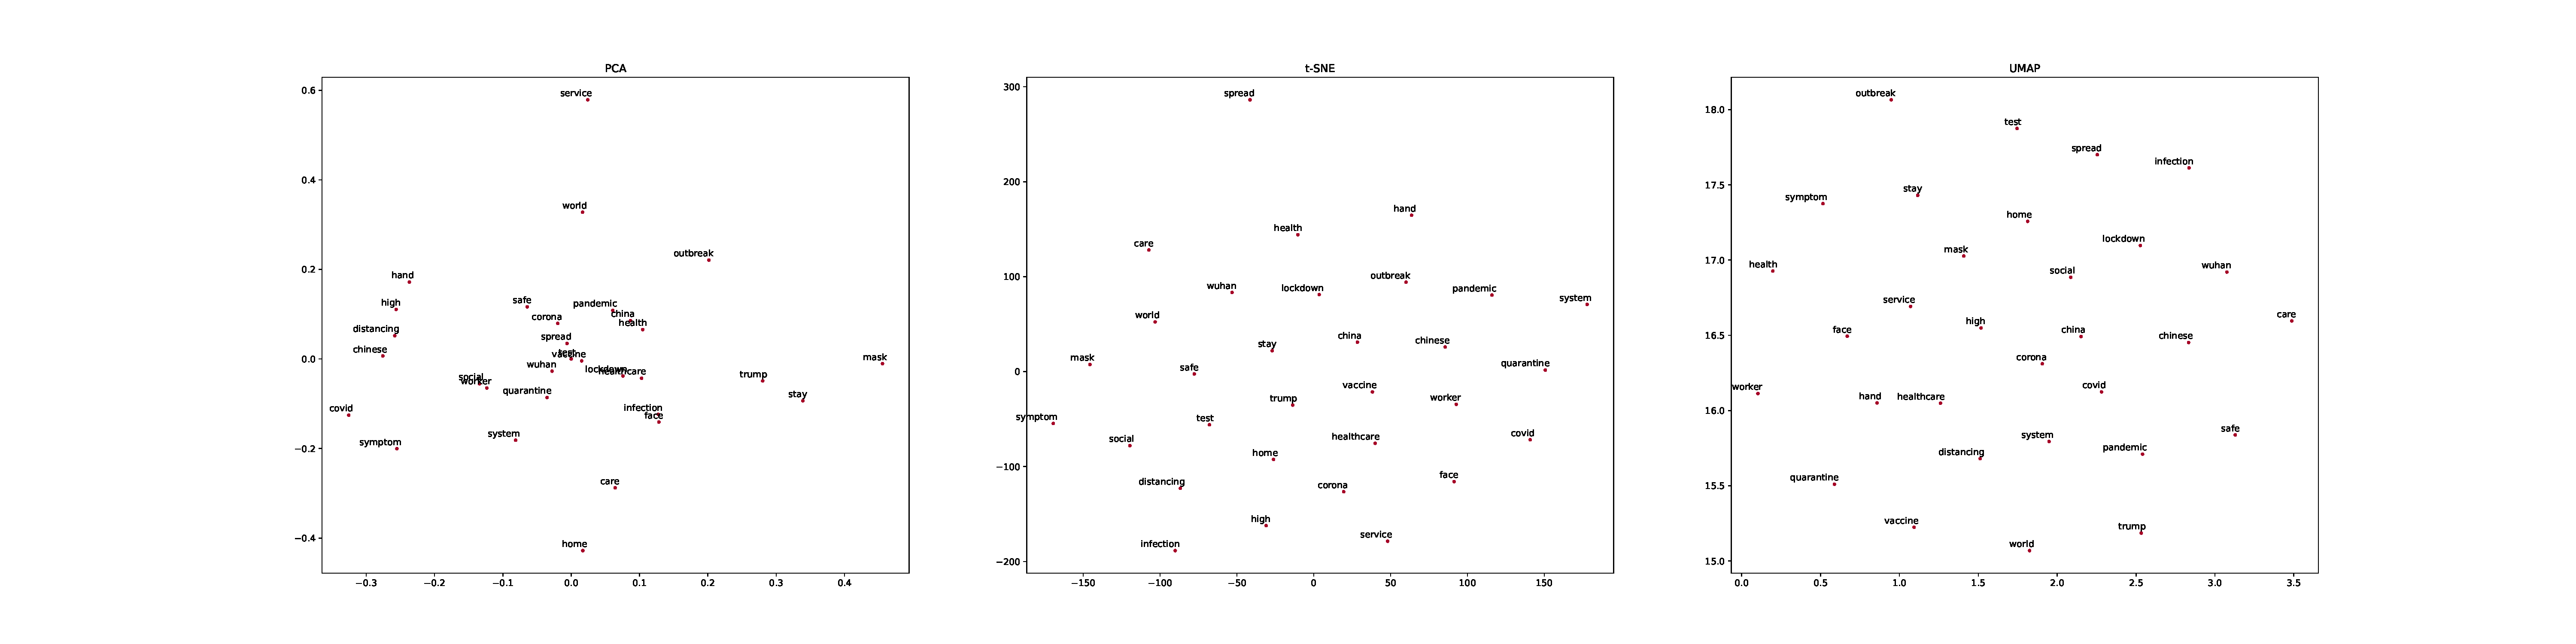
\includegraphics[width=1\textwidth]{images/keywords_bow.pdf}
  \caption{Distribution of keywords used to select tweets for the TweetsCOV19 dataset.}
 \label{fig:bow_key}
 \end{subfigure}
 \centering
 \begin{subfigure}{\columnwidth}
 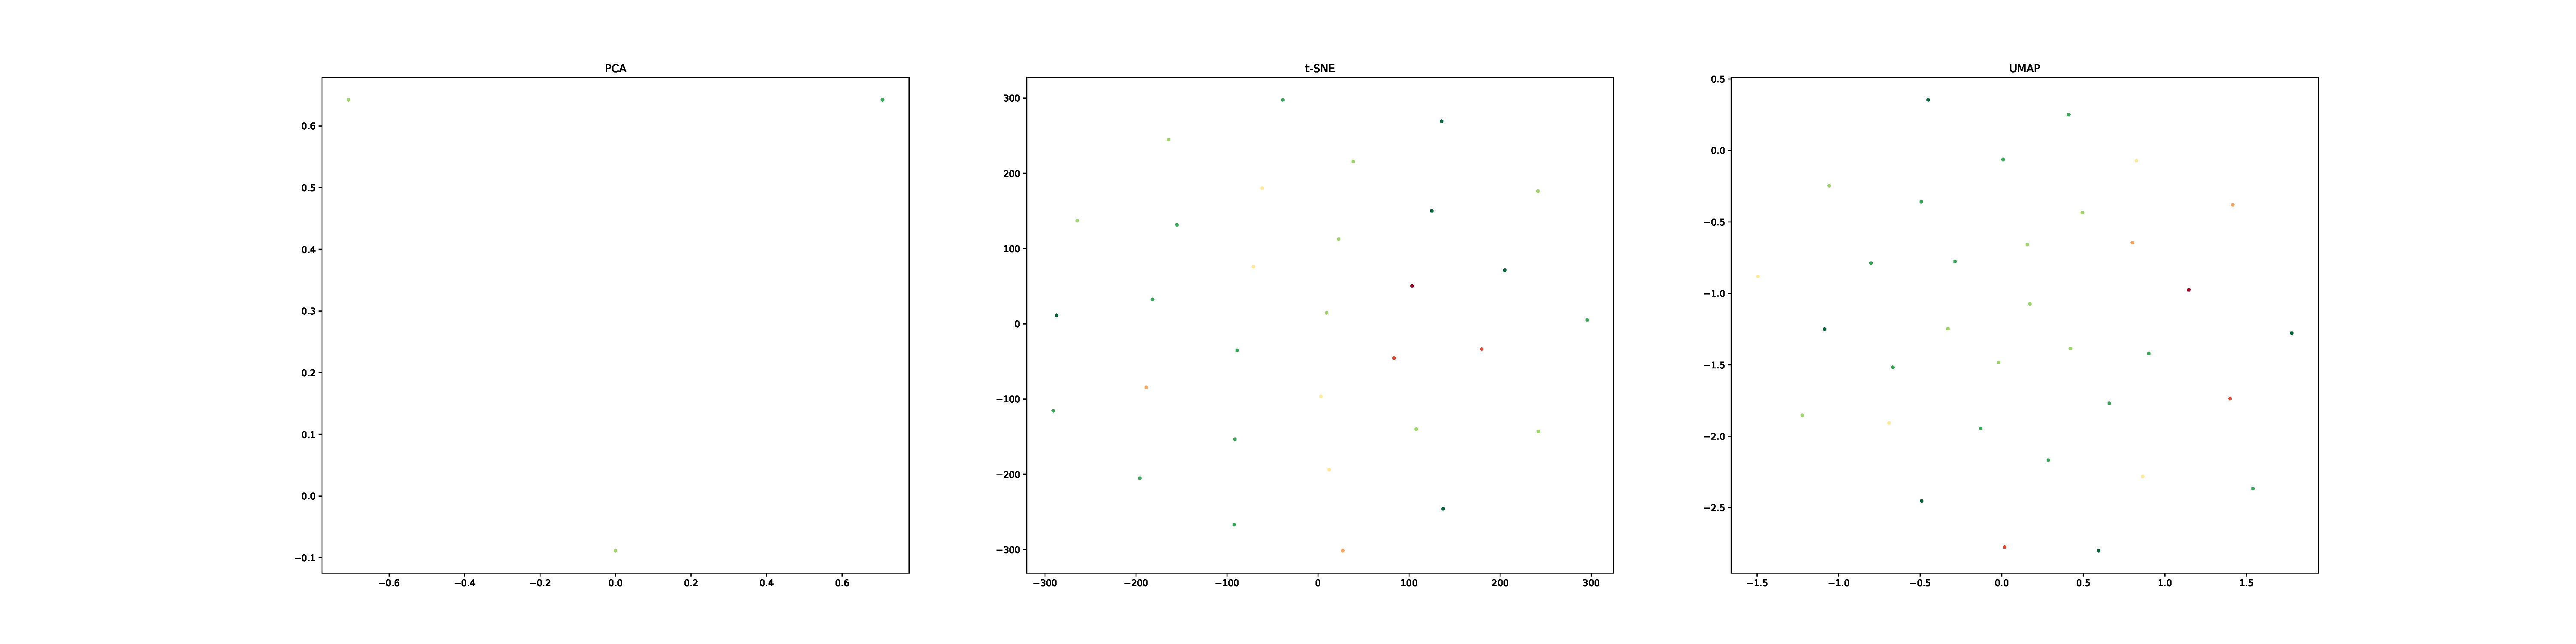
\includegraphics[width=1\textwidth]{images/keywords_bow_posneg.pdf}
  \caption{Distribution of positive and negative words from the AFINN-96 dataset.}
  \label{fig:bow_posneg}
 \end{subfigure}
 \caption{Visualization of BoW embedding of keywords and positive/negative words with PCA, t-SNE, and UMAP.}
 \label{fig:bow_viz}
\end{figure}

\begin{figure}
 \centering
 \begin{subfigure}{\columnwidth}
 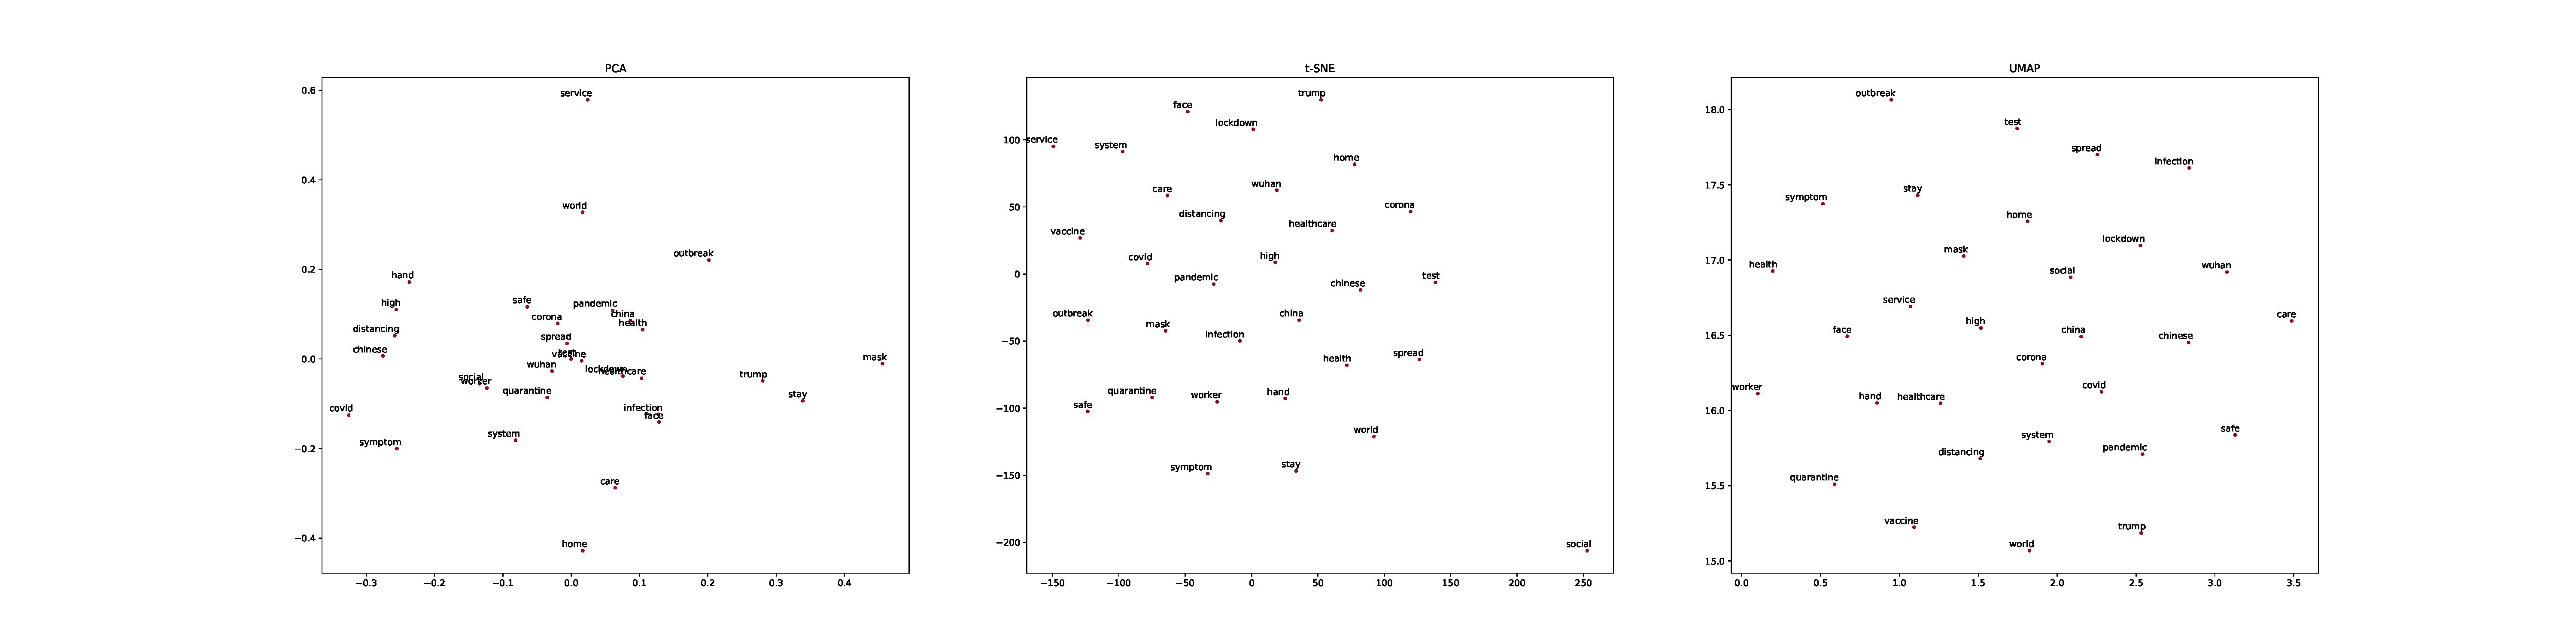
\includegraphics[width=1\textwidth]{images/keywords_tfidf.pdf}
 \caption{Distribution of keywords used to select tweets for the TweetsCOV19 dataset.}
 \label{fig:tfidf_key}
 \end{subfigure}
 \centering
 \begin{subfigure}{\columnwidth}
 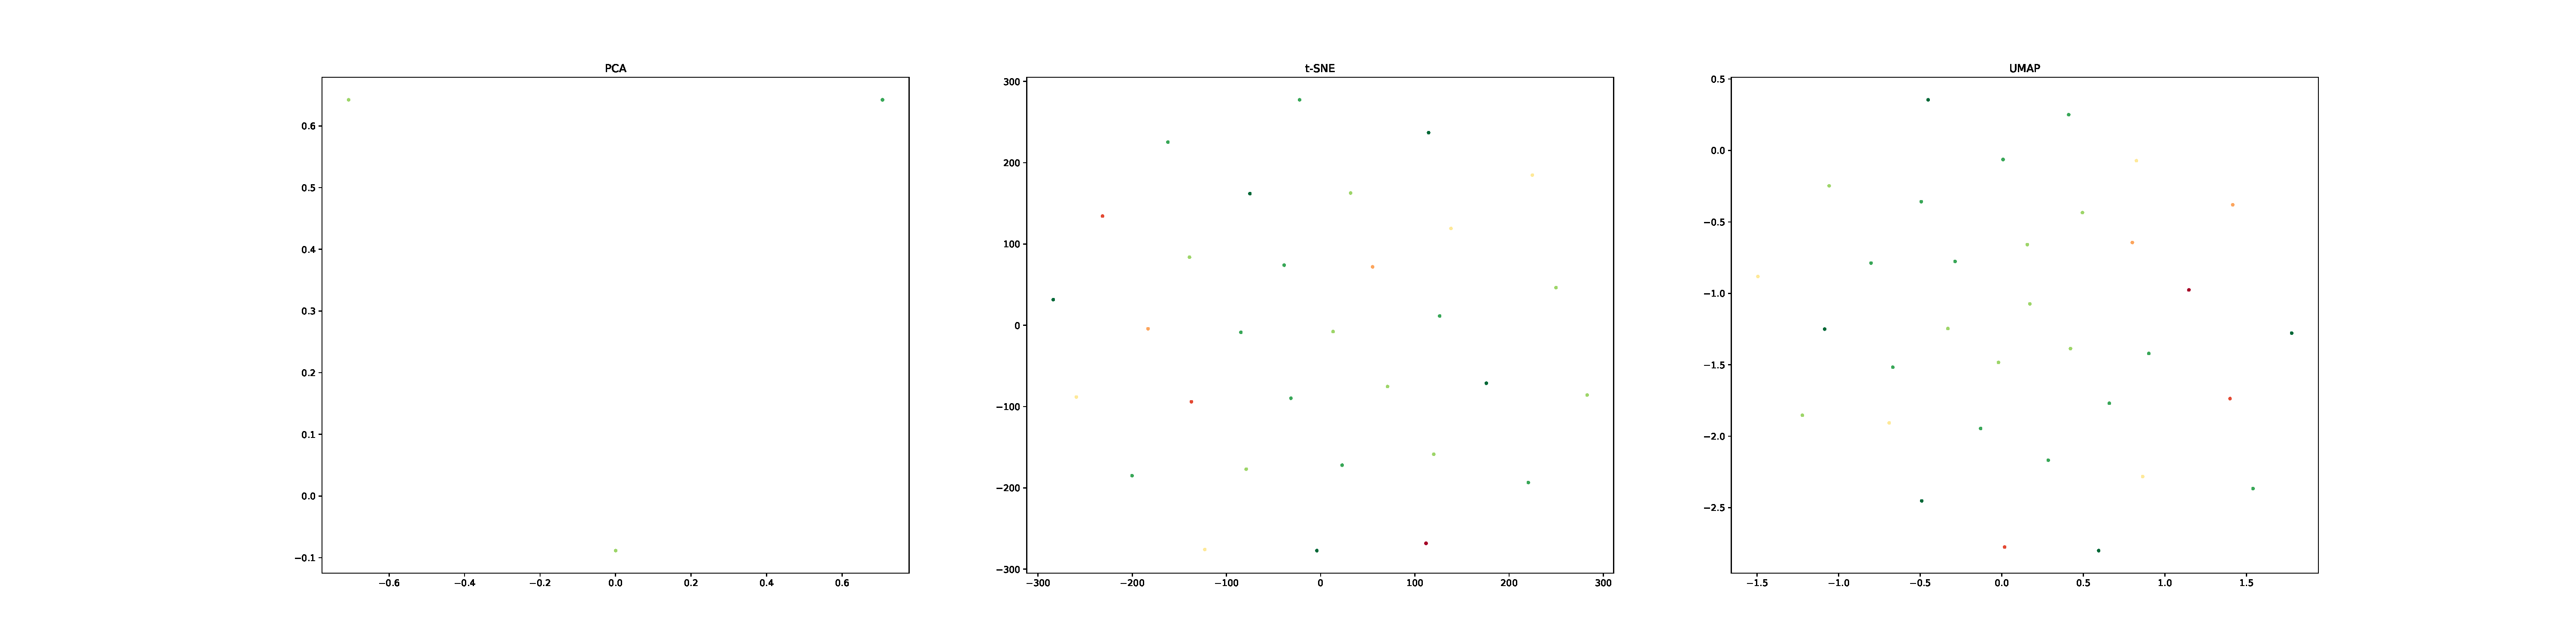
\includegraphics[width=1\textwidth]{images/keywords_tfidf_posneg.pdf}
 \caption{Distribution of positive and negative words from the AFINN-96 dataset.}
  \label{fig:tfidf_posneg}
 \end{subfigure}
 \caption{Visualization of TF-IDF embedding of keywords and positive/negative words with PCA, t-SNE, and UMAP.}
 \label{fig:tfidf_viz}
\end{figure}

\begin{figure}
 \centering
 \begin{subfigure}{\columnwidth}
 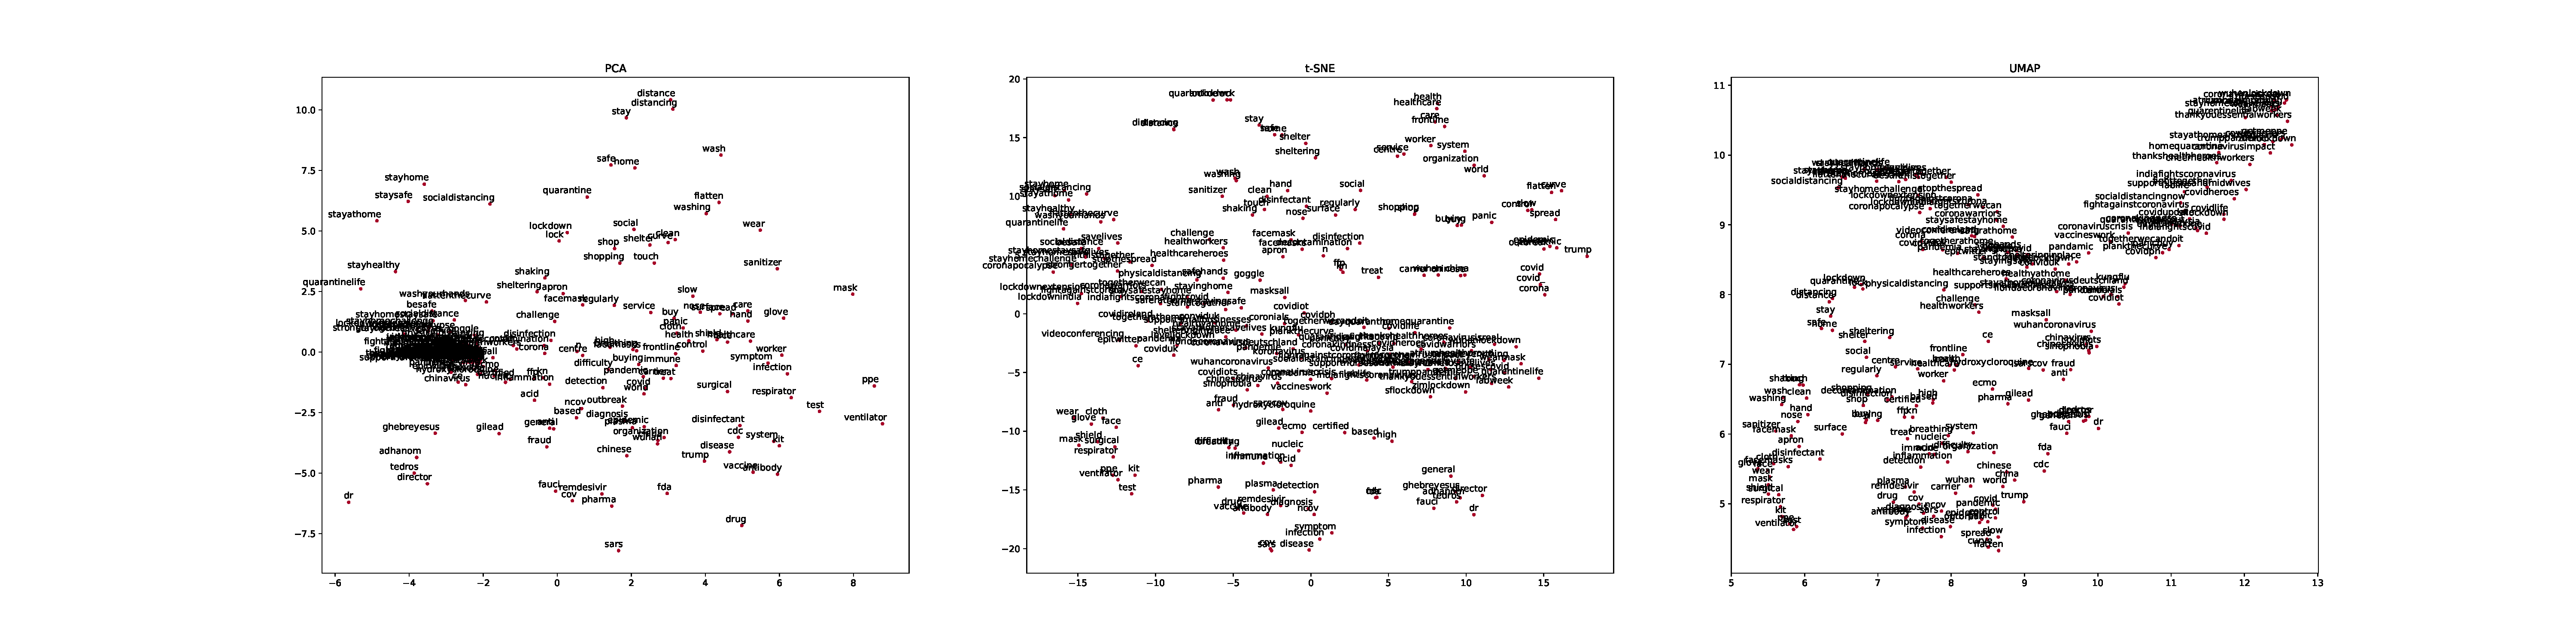
\includegraphics[width=1\textwidth]{images/keywords_cbow.pdf}
 \caption{Distribution of keywords used to select tweets for the TweetsCOV19 dataset.}
 \label{fig:cbow_key}
 \end{subfigure}
 \centering
 \begin{subfigure}{\columnwidth}
 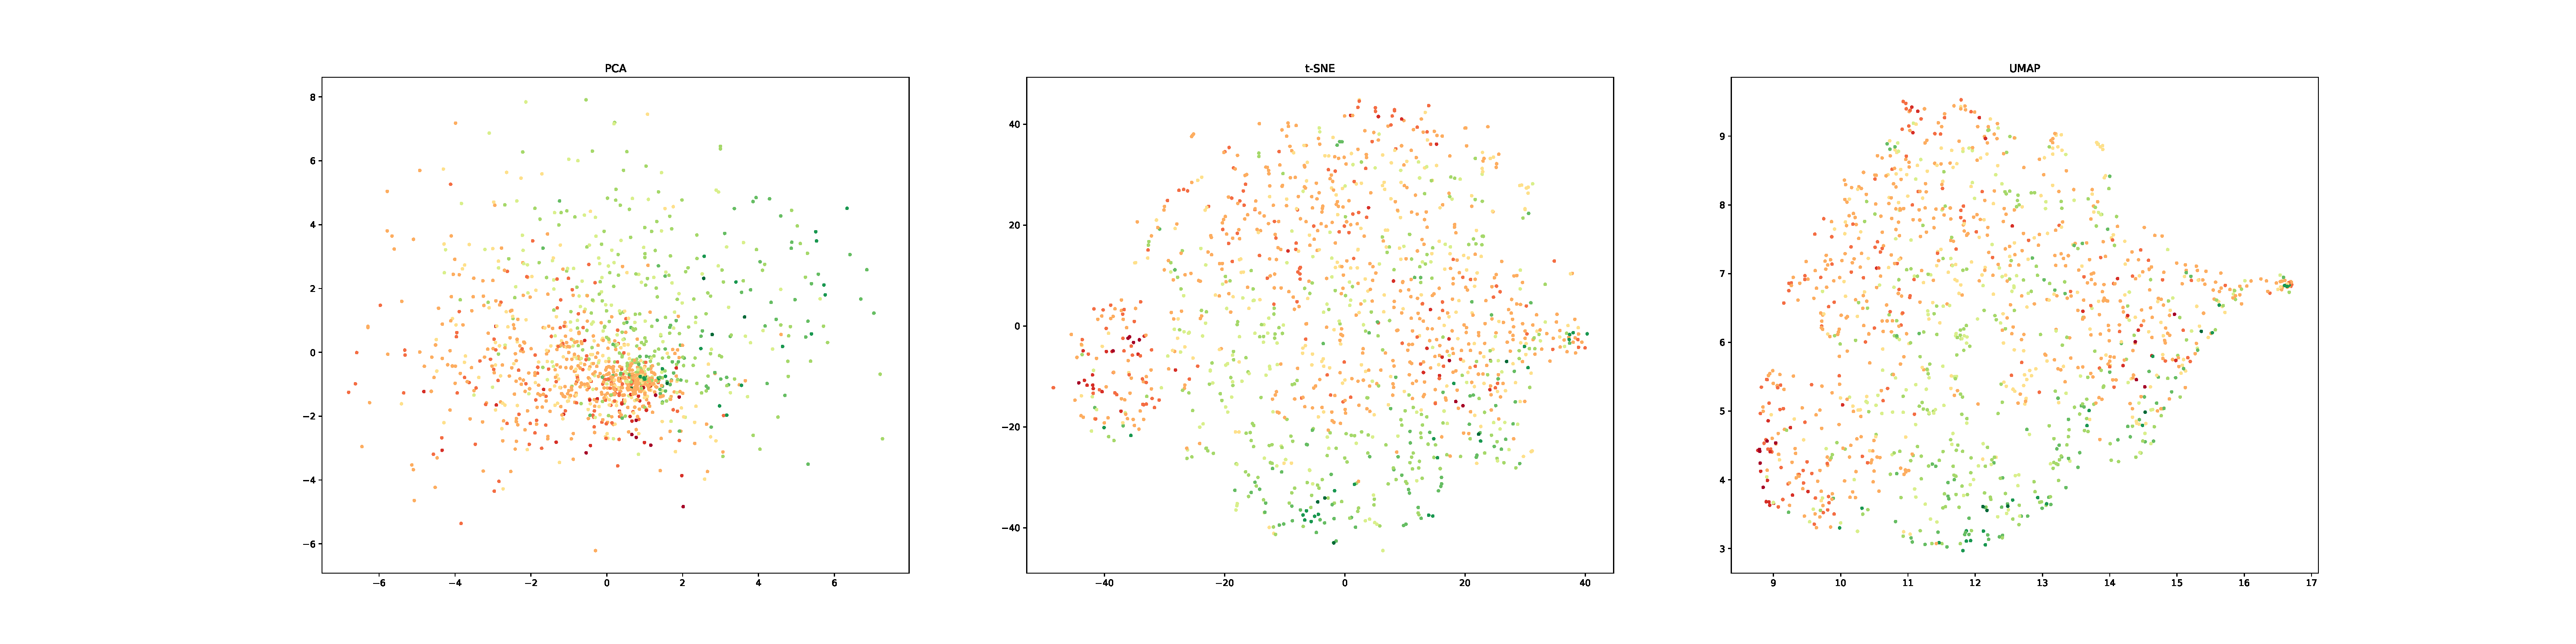
\includegraphics[width=1\textwidth]{images/keywords_cbow_posneg.pdf}
 \caption{Distribution of positive and negative words from the AFINN-96 dataset.}
  \label{fig:cbow_posneg}
 \end{subfigure}
 \caption{Visualization of CBOW embedding of keywords and positive/negative words with PCA, t-SNE, and UMAP.}
 \label{fig:cbow_viz}
\end{figure}

\begin{figure}
 \centering
 \begin{subfigure}{\columnwidth}
 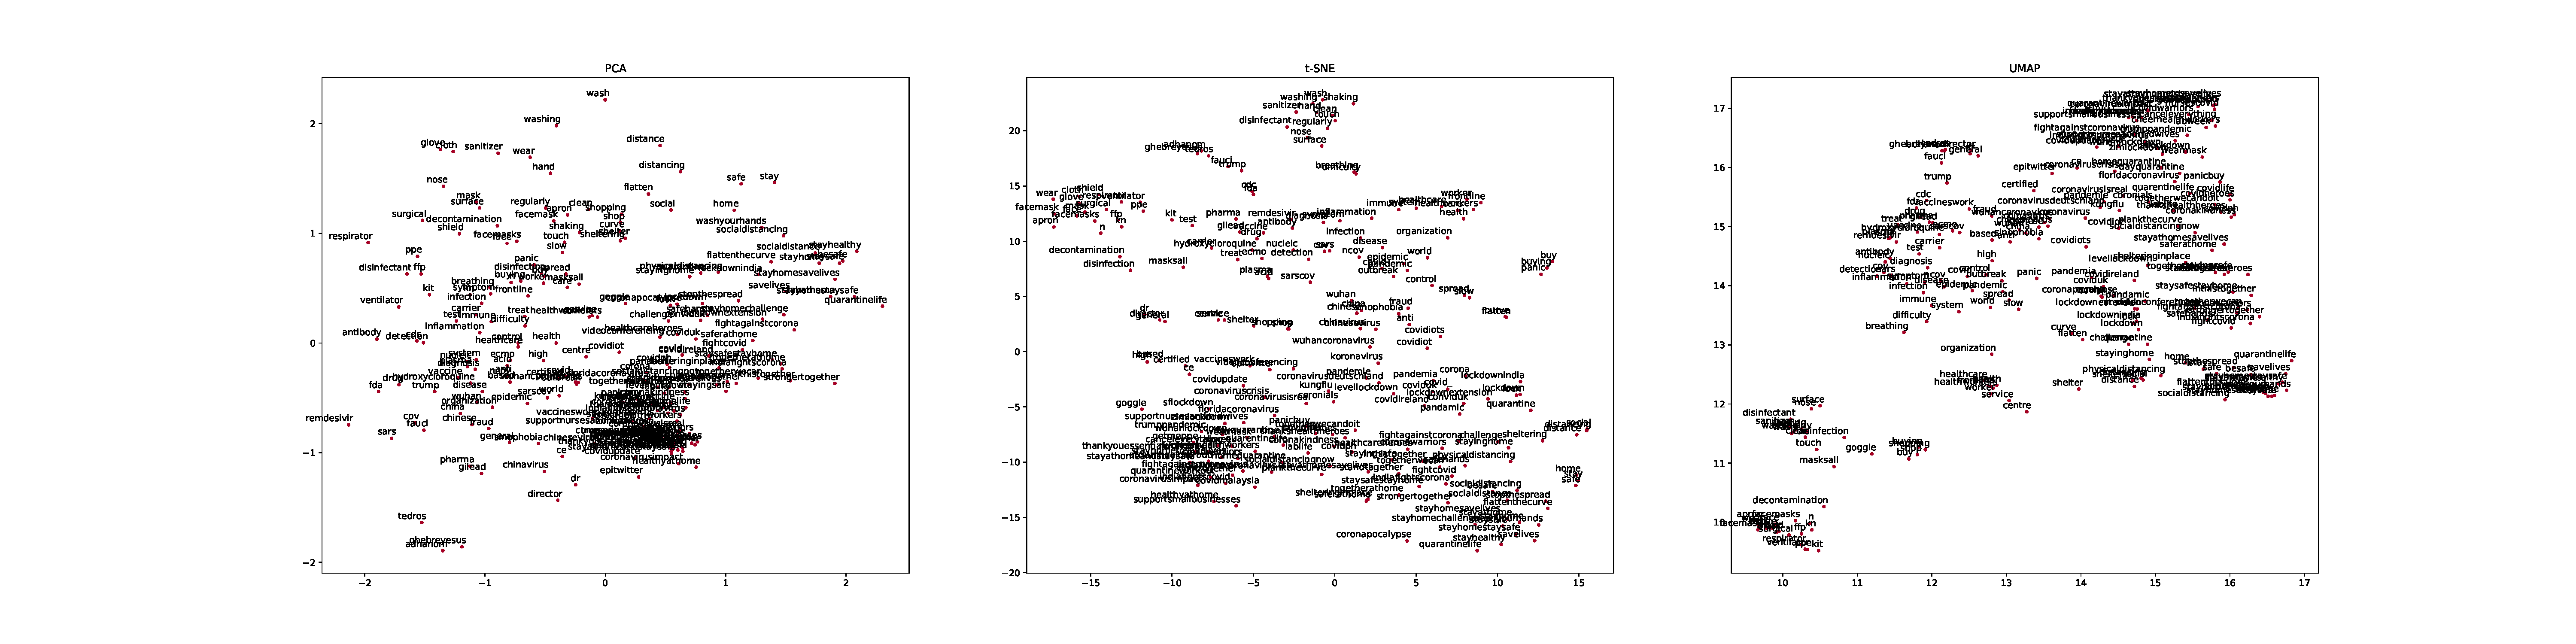
\includegraphics[width=1\textwidth]{images/keywords_sgram.pdf}
 \caption{Distribution of keywords used to select tweets for the TweetsCOV19 dataset.}
 \label{fig:sgram_key}
 \end{subfigure}
 \centering
 \begin{subfigure}{\columnwidth}
 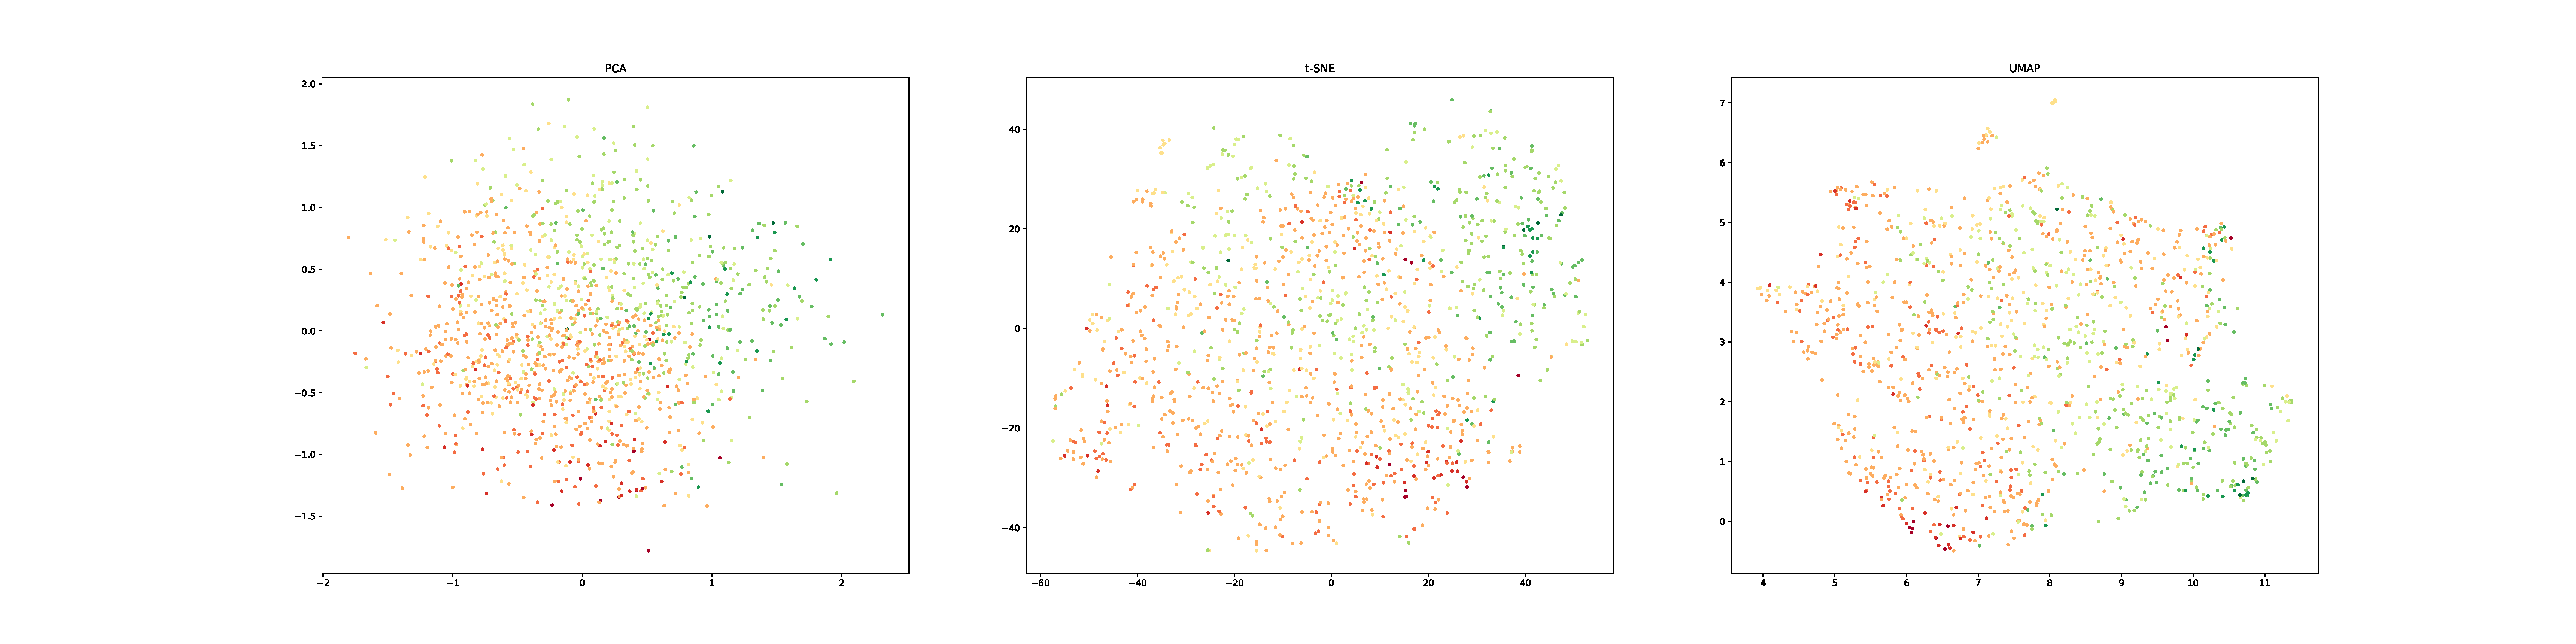
\includegraphics[width=1\textwidth]{images/keywords_sgram_posneg.pdf}
 \caption{Distribution of positive and negative words from the AFINN-96 dataset.}
  \label{fig:sgram_posneg}
 \end{subfigure}
 \caption{Visualization of Skip-gram embedding of keywords and positive/negative words with PCA, t-SNE, and UMAP.}
 \label{fig:sgram_viz}
\end{figure}

\begin{figure}
 \centering
 \begin{subfigure}{\columnwidth}
 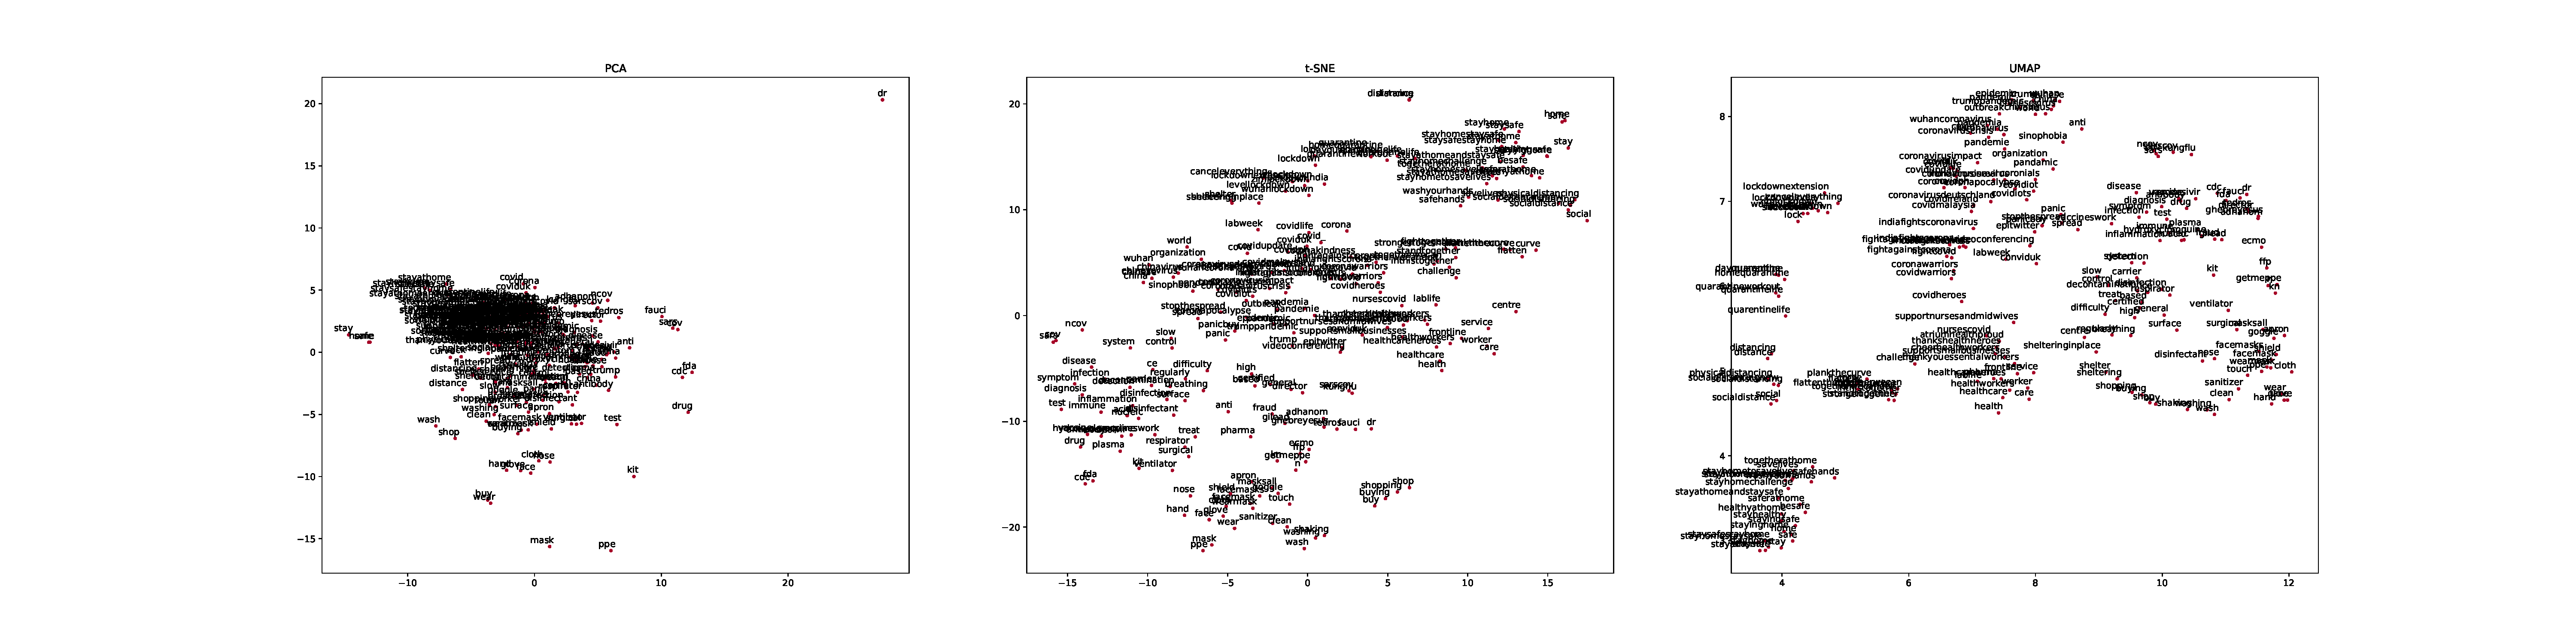
\includegraphics[width=1\textwidth]{images/keywords_ft.pdf}
 \caption{Distribution of keywords used to select tweets for the TweetsCOV19 dataset.}
 \label{fig:ft_key}
 \end{subfigure}
 \centering
 \begin{subfigure}{\columnwidth}
 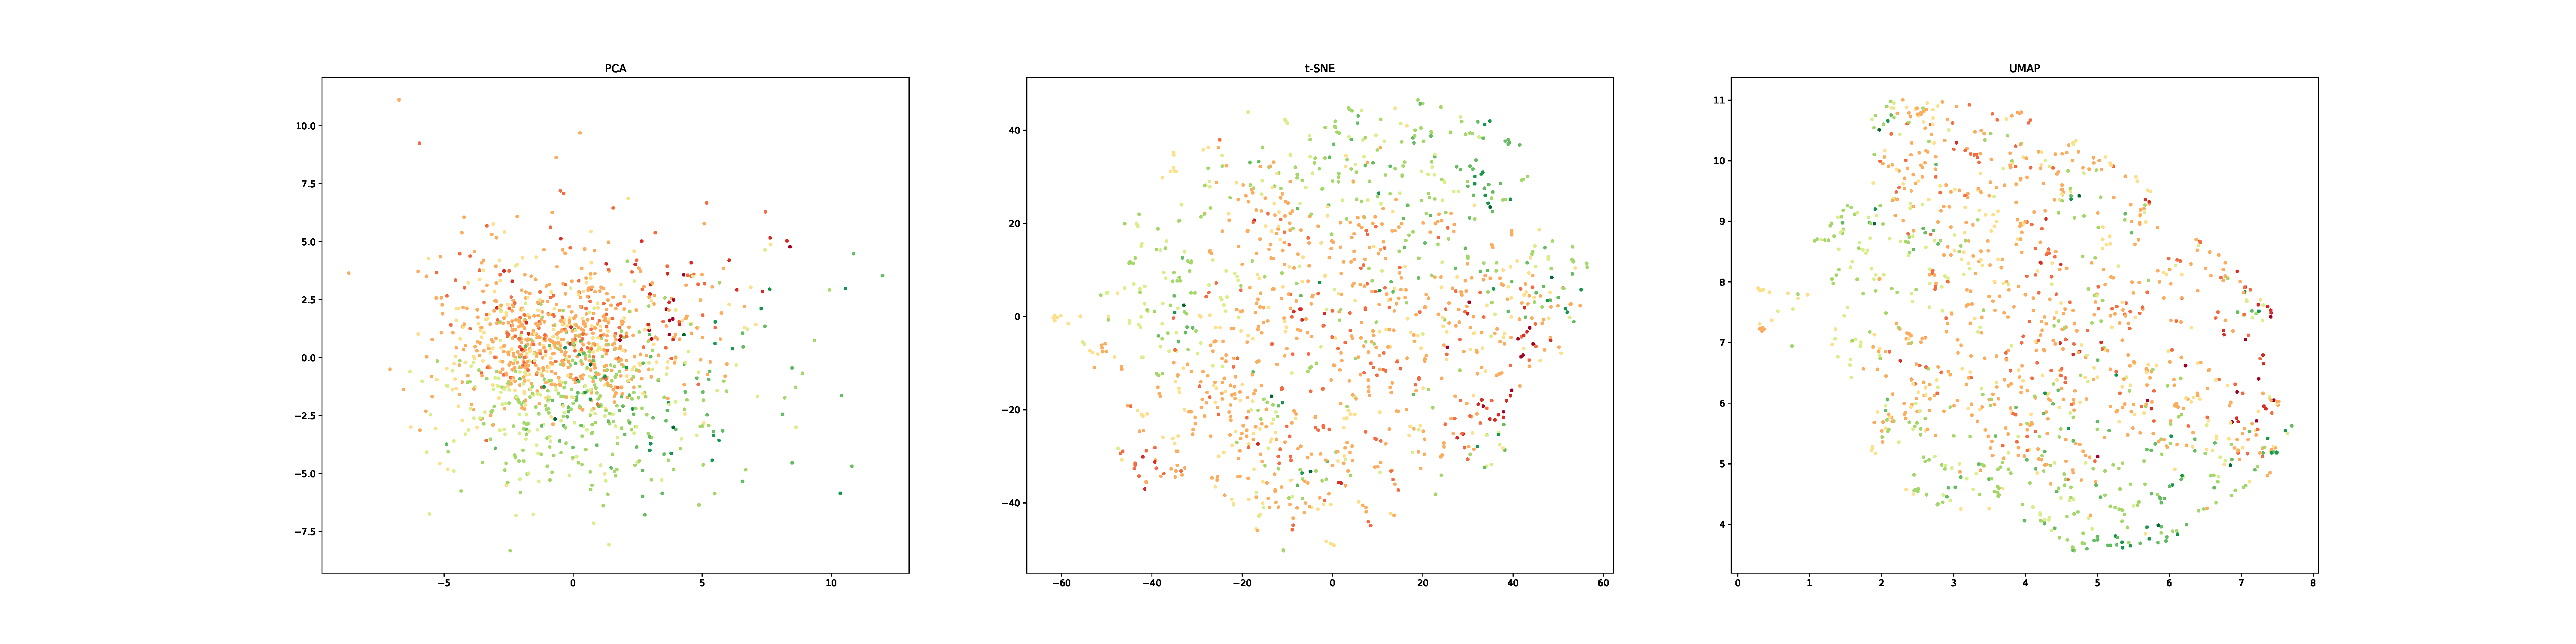
\includegraphics[width=1\textwidth]{images/keywords_ft_posneg.pdf}
 \caption{Distribution of positive and negative words from the AFINN-96 dataset.}
  \label{fig:ft_posneg}
 \end{subfigure}
 \caption{Visualization of FastText embedding of keywords and positive/negative words with PCA, t-SNE, and UMAP.}
 \label{fig:ft_viz}
\end{figure}

\begin{figure}
 \centering
 \begin{subfigure}{\columnwidth}
 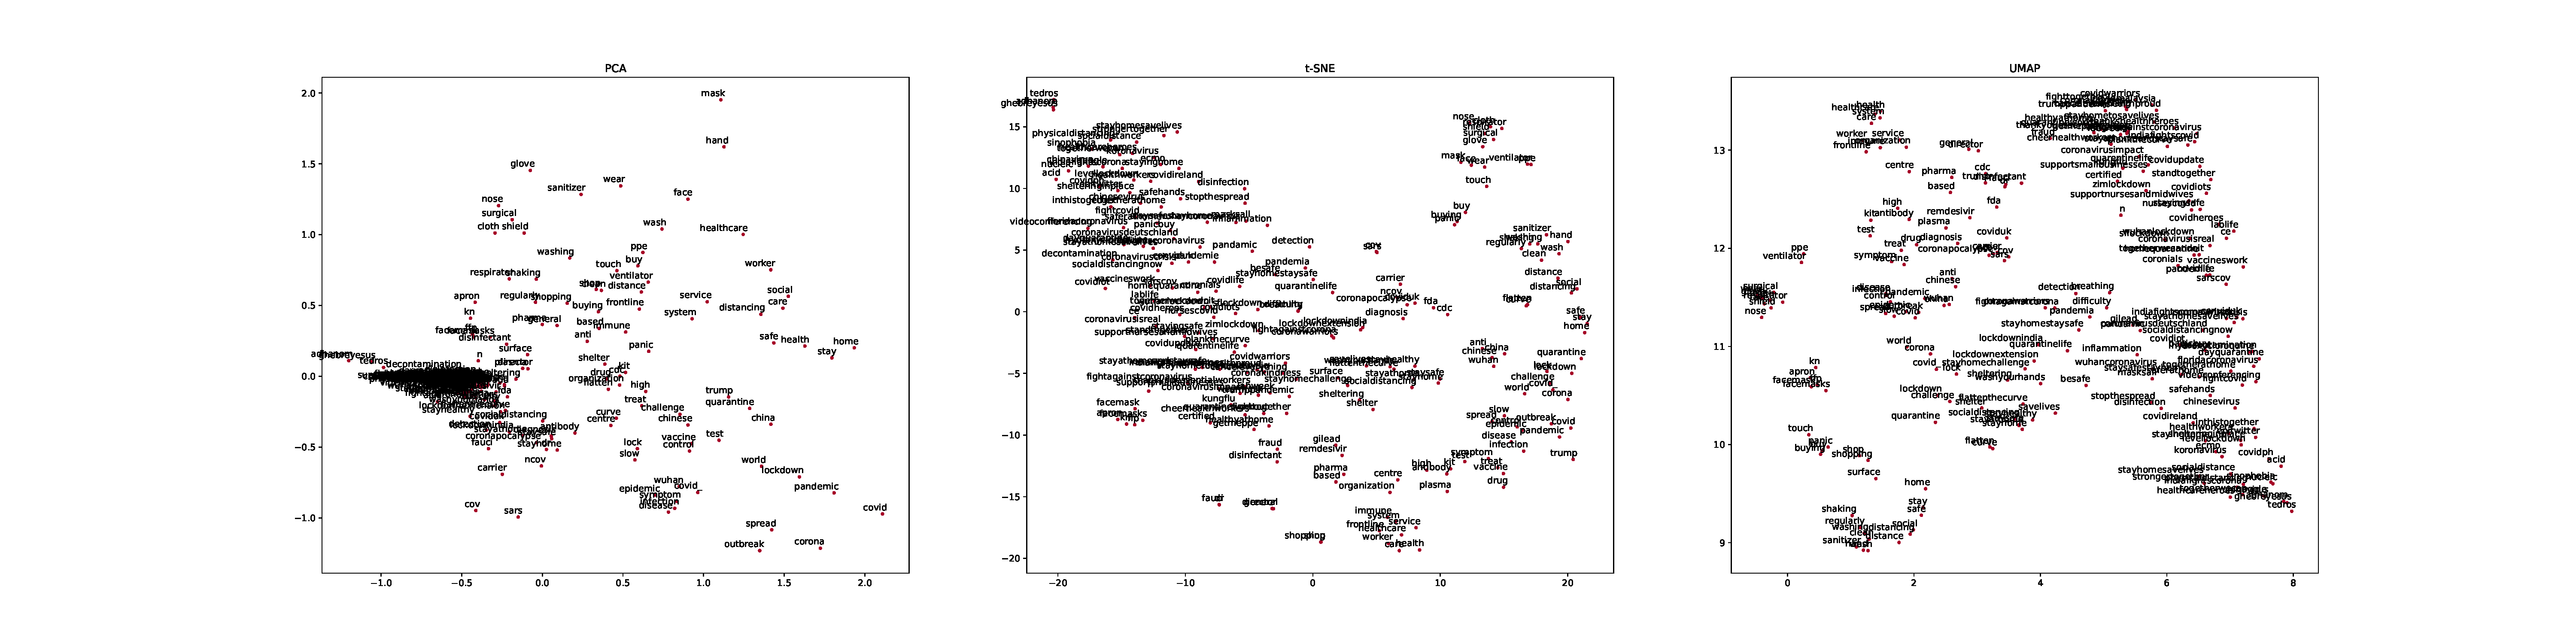
\includegraphics[width=1\textwidth]{images/keywords_glove.pdf}
 \caption{Distribution of keywords used to select tweets for the TweetsCOV19 dataset.}
 \label{fig:glove_key}
 \end{subfigure}
 \centering
 \begin{subfigure}{\columnwidth}
 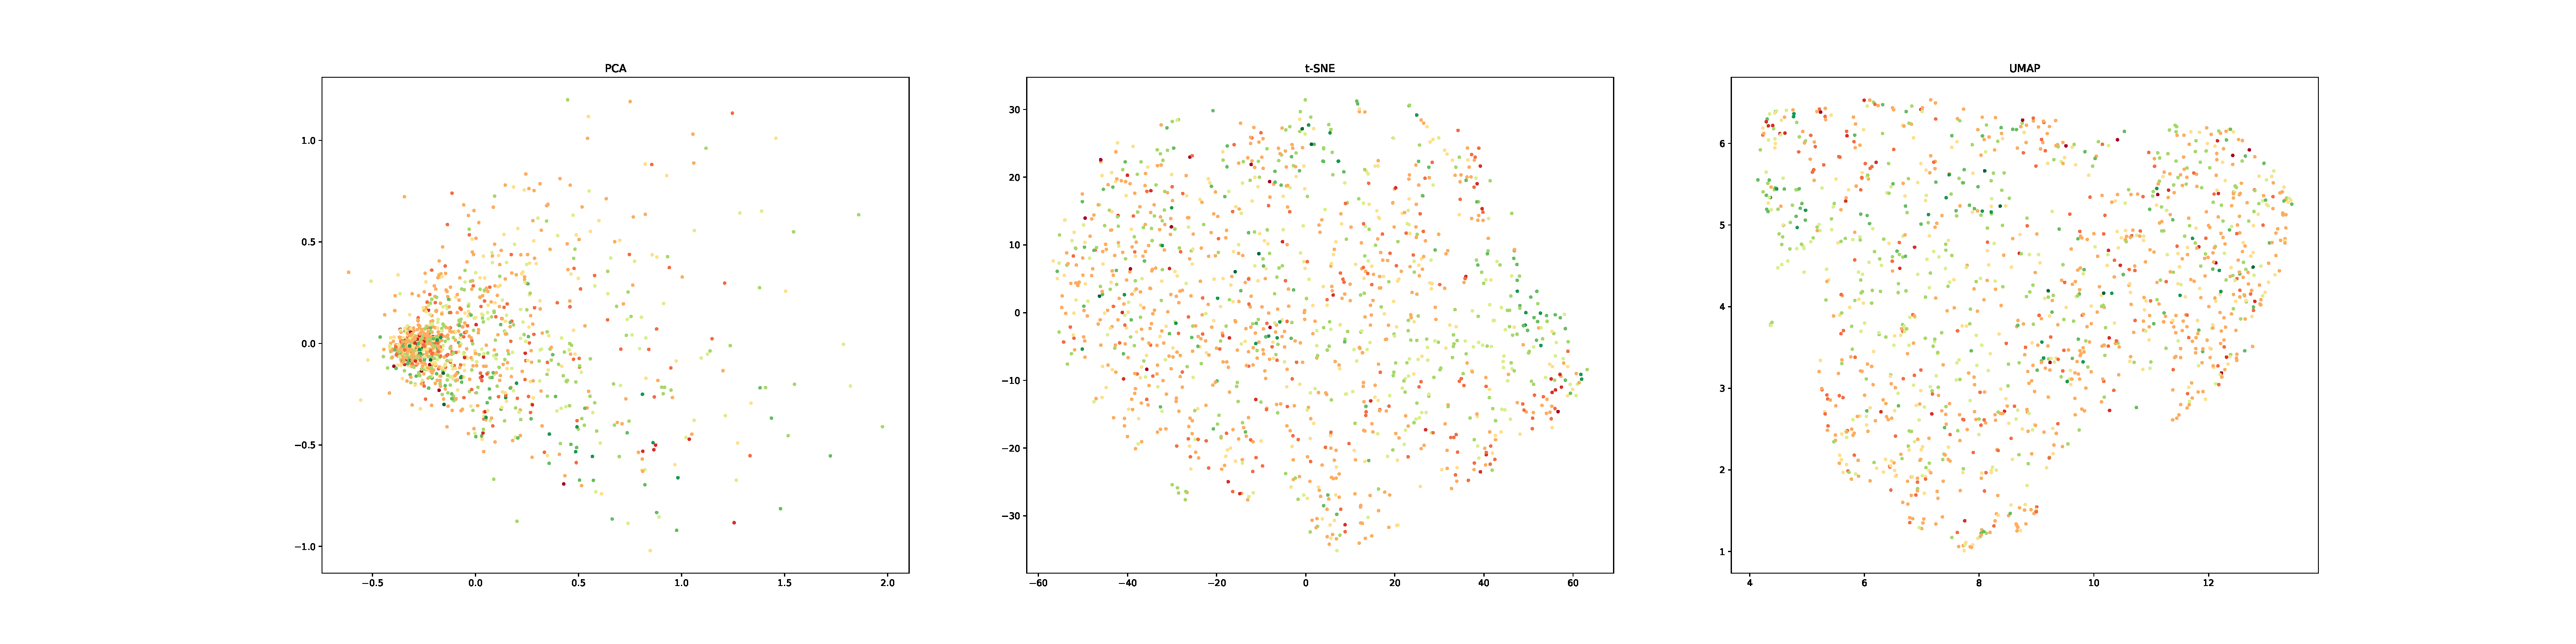
\includegraphics[width=1\textwidth]{images/keywords_glove_posneg.pdf}
 \caption{Distribution of positive and negative words from the AFINN-96 dataset.}
  \label{fig:glove_posneg}
 \end{subfigure}
 \caption{Visualization of Glove embedding of keywords and positive/negative words with PCA, t-SNE, and UMAP.}
 \label{fig:glove_viz}
\end{figure}

After embedding of keywords with FastText, we can see a clear grouping of similar words when visualized with t-SNE and especially UMAP, as can be seen in Figure \ref{fig:ft_key}. This makes sense, since FastTexts looks at the morphological similarity of words by working with n-grams. For example, in the UMAP visualization, 'distancing' and 'distance' are grouped together, but 'physicaldistancing', 'socialdistancing', and 'socialdistance' are also located nearby. This will likely make it easier for FastText to assign similar scores to similar words, e.g. to 'bad' and 'badly'.

Embeddings with GloVe, Skip-grams, and CBOW seem to capture more subtle relationships, and UMAP visualization is able to group words such as 'facemask', 'kn', and 'ffp' together. The visualizations can be found in Figures \ref{fig:glove_key}, \ref{fig:sgram_key}, and \ref{fig:cbow_key}. Classification results using any of these embedding models will therefore in all likelihood be relatively similar. 

Application of PCA on the embedding with CBOW, Skip-grams, and FastText seems to show a reasonable separation of positive and negative words, although the t-SNE and UMAP visualizations do not noticeably confirm this finding (see Figure \ref{fig:cbow_posneg}, \ref{fig:ft_posneg}, and \ref{fig:sgram_posneg}). GloVe embedding, on the other hand, seems to not be easily separable in two dimensions after application of PCA, but shows similar results for t-SNE and UMAP, as can be seen in Figure \ref{fig:glove_posneg}.
In general, we can see that most of embedding models are able to pick up on the sentiments of certain words, but not on the relative weights of that sentiment. Therefore, it might be difficult for our downstream classifiers to pick up on these nuances, and especially so when using GloVe embeddings.

\subsection*{Q7: Tweet embeddings (2 pts)}
\textit{Propose three different approaches to combine word embeddings into an embedding for each tweet. Provide a code snippet for each function. How do all of the above methods deal with out-of-vocabulary words?}

For this question, we compare summing, averaging, and concatenation of the minimum and maximum of the word embeddings.

Our 'summing' method simply consists of summing up the embeddings of every word in the tweet. If a word cannot be found in the vocabulary, we do not include it in the sum (this is done because we limited vocabulary size in some of our methods for computational reasons).

The 'averaging' method uses the results from the first 'summing' method, but divides it by the number of valid (i.e. not OOV) words found in the tweet.

The code for the first two methods can be found in Code Snippet \ref{listing:p2-sumav}.

\begin{listing*}
\begin{minted}{python}
def av_sum_sentence(row, model, vec_size=vec_size, av=True):
    if row != []:
        red = 0
        sentence = 0
        for word in row:
            try:
                sentence += model.wv[word]
            except:
                red += 1
        if av:
            sentence = sentence/(1+len(row)-red)
        if red == len(row):
            return np.zeros(vec_size).tolist()
        else:
            return sentence.tolist()
    else:
        return np.zeros(vec_size).tolist()


def av_sum_sentence_bow(row, vectorizer, transformer=None, av=True):
    sentence = vectorizer.transform([row])
    if transformer is not None:
        sentence = transformer.transform(sentence)
    sentence = sentence.toarray()[0]
    if av:
        sentence = sentence/(1+sentence.sum())
    return sentence.tolist()
\end{minted}
\caption{Code of our 'summing' and 'averaging' word-to-sentence embedding functions. We created two functions to account for the individual differences between Gensim \cite{gensim} and scikit-learn \cite{sklearn1, sklearn2}.}
\label{listing:p2-sumav}
\end{listing*}

Finally, we designed a 'minmax' method, where we find the respective minimum and maximum values (per index) of all word embeddings and concatenate the results. Again, as can be seen in Code Snippet \ref{listing:p2-minmax}, if a word is OOV, we simply ignore it.

\begin{listing*}
\begin{minted}{python}
def minmax_sentence(row, model, vec_size=vec_size):
    sentence_min = np.ones(vec_size)*1000
    sentence_max = np.ones(vec_size)*(-1000)
    if row != []:
        red = 0
        for word in row:
            try:
                sentence_min = np.minimum(np.asarray(model.wv[word]), sentence_min[idx])
                sentence_max = np.maximum(np.asarray(model.wv[word]), sentence_max[idx])
            except:
                red += 1
        if red == len(row):
            sentence_min = np.ones(vec_size)*1000
            sentence_max = np.ones(vec_size)*(-1000)
    return np.concatenate((sentence_min, sentence_max), axis=0).tolist()

def minmax_sentence_bow(row, vectorizer, vocab_size, transformer=None):
    sentence_min = np.ones(vocab_size)
    sentence_max = np.zeros(vocab_size)
    
    if row != []:
        res = vectorizer.transform([row])
        if transformer is not None:
            res = transformer.transform(res)
        sentence_min = np.minimum(res.toarray()[0], sentence_min)
        sentence_max = np.maximum(res.toarray()[0], sentence_max)
    return np.concatenate((sentence_min, sentence_max), axis=0).tolist()
\end{minted}
\caption{Code of our 'minmax' word-to-sentence embedding function. There are two functions, in order to account for the differences between the Gensim \cite{gensim} and scikit-learn libraries \cite{sklearn1, sklearn2}.}
\label{listing:p2-minmax}
\end{listing*}


\subsection*{Q8: Classifier (3 pts)}
\textit{Implement three downstream classifiers to perform sentiment analysis of your tweets (i.e., predict both the positive (1 to 5) and negative (-1 to -5) sentiment score for each tweet). For each classifier, briefly explain how it works and make sure to tune hyper-parameters appropriately. Provide a results table showcasing the performance of all tested classifiers for each embeddings approach you implemented in Q1-5, and each aggregation method in Q7. For each family of classifiers tested provide a code snippet.}

Instead of classifiers, we implement three regression models to perform sentiment analysis of the tweets, since the labels 'positive sentiment score' and 'negative sentiment score' are ordered discrete values. We compare our results using the mean harmonic F1 score (i.e. the mean of the harmonic F1 score for positive and negative sentiments respectively).

Before calculating the harmonic F1 score, we round the regression output to the nearest integer, and then clip all values outside of the sentiment score range (1 to 5 for positive sentiments, and -5 to -1 for negative sentiments), to ensure consistency with classifier outputs. This details of this preprocessing step can be found in Code Snippet \ref{listing:f1}

\begin{listing*}
\begin{minted}{python}
from sklearn.metrics import f1_score, make_scorer

def weighted_harmonic_f1_score(y_true, y_pred):
    y_pred_pos = np.clip(np.around(y_pred[:,0]), 1, 5).astype(int)
    y_pred_neg = np.clip(np.around(y_pred[:,1]), -5, -1).astype(int)
    f1_scores_pos = f1_score(y_true[:,0], y_pred_pos, average='weighted')
    f1_scores_neg = f1_score(y_true[:,1], y_pred_neg, average='weighted')
    weighted_f1 = (f1_scores_pos + f1_scores_neg)/2
    return weighted_f1

weighted_harmonic_f1_scorer = make_scorer(weighted_harmonic_f1_score)

\end{minted}
\caption{Code snippet showing the calculation of the weighted harmonic F1 score used in Q8.}
\label{listing:f1}
\end{listing*}


All hyperparameter tuning was performed using GridSearchCV from the scikit-learn library \cite{sklearn1, sklearn2}. Still, to speed up training, we tune the models with limited parameters and train on only two folds.

For our first 'classifier', we use Random Forests \cite{randomforest}. Random Forests is a model that combines the results of multiple decision trees, returning the most likely class for classification, or the mean prediction for regression. The code can be found in Code Snippet \ref{listing:p2-randomforest}.

\begin{listing*}
\begin{minted}{python}
from sklearn.ensemble import RandomForestRegressor
from sklearn.model_selection import GridSearchCV
from sklearn.multioutput import MultiOutputRegressor


def rand_forest(sentence, sentence_test):
    params = {'estimator__n_estimators':[5,15],
              'estimator__n_jobs':[-1], 'estimator__random_state':[42],
              'estimator__criterion':['squared_error'], 'estimator__max_depth':[4,5],
              'estimator__verbose':[0]}
    regr = GridSearchCV(MultiOutputRegressor(RandomForestRegressor()), param_grid=params,
                        n_jobs=-1, cv=2, scoring=weighted_harmonic_f1_scorer, verbose=0)
    start_time = time.time()
    regr.fit(sentence, np.asarray(y_train_val[['pos_sent', 'neg_sent']].values.tolist()))
    elapsed_time = time.time() - start_time

\end{minted}
\caption{Code snippet for the first classifier, Random Forests.}
\label{listing:p2-randomforest}
\end{listing*}

For the second 'classifier', we use GradientBoosting \cite{gradboost1, gradboost2, gradboost3}. Gradient boosting is a method that combines weak models to create a strong predictive model. It does so by iteratively improving upon the loss from the weak model of the previous round.
We again use a method from scikit-learn \cite{sklearn1, sklearn2}, as you can see in \ref{listing:p2-gradboost}.

\begin{listing*}
\begin{minted}{python}
from sklearn.ensemble import GradientBoostingRegressor

def grad_reg(sentence, sentence_test):
    params = {'estimator__learning_rate': [0.1, 1], 'estimator__n_estimators': [5, 15],
              'estimator__max_depth': [4, 5], 'estimator__n_iter_no_change':[7]}
    regr = GridSearchCV(MultiOutputRegressor(GradientBoostingRegressor()), param_grid=params,
                        n_jobs=-1, cv=2, scoring=weighted_harmonic_f1_scorer, verbose=0)
    start_time = time.time()
    regr.fit(sentence, np.asarray(y_train_val[['pos_sent', 'neg_sent']].values.tolist()))
    elapsed_time = time.time() - start_time
\end{minted}
\caption{Code snippet for the second classifier, Gradient Boosting.}
\label{listing:p2-gradboost}
\end{listing*}

Finally, for our third 'classifier', we implemented AdaBoost \cite{adaboost} in Code Snippet \ref{listing:p2-adaboost}. Adaptive boosting is an iterative training method that in every iteration adjusts the weights of  the data points that were predicted badly in the previous iteration. The final output is the weighted average of all previous models, the weights depending on their overall performance.

\begin{listing*}
\begin{minted}{python}
from sklearn.ensemble import AdaBoostRegressor

def ada_reg(sentence, sentence_test):
    params = {'estimator__loss': ['square', 'exponential'], 'estimator__n_estimators': [5, 15, 30],
              'estimator__learning_rate': [0.1, 1, 10], 'estimator__random_state':[42]}
    regr = GridSearchCV(MultiOutputRegressor(AdaBoostRegressor()), param_grid=params,
                        n_jobs=-1, cv=2, scoring=weighted_harmonic_f1_scorer, verbose=0)
    start_time = time.time()
    regr.fit(sentence, np.asarray(y_train_val[['pos_sent', 'neg_sent']].values.tolist()))
    elapsed_time = time.time() - start_time
\end{minted}
\caption{Code snippet for the third classifier, AdaBoost.}
\label{listing:p2-adaboost}
\end{listing*}

The train and test scores of the classifiers for each word embedding model and aggregation method can be found in Table \ref{table:score}. 

\subsection*{Q9: Performance comparison (3 pts)}
\textit{Using the summary table computed in Q8, compare the performance of all methods on the sentiment analysis task using the TweetsCOV19 dataset. Also compare methods from a computational point of view. What embedding model, aggregation method and classifier would you select among all approaches? Give potential extensions that could help improve your performance.}

\begin{table}[]
\resizebox{\textwidth}{!}{%
\begin{tabular}{|l|lll|l|l|lll|}
\cline{1-4} \cline{6-9}
\textbf{TRAIN SCORE} & RandomForests & GradientBoosting & AdaBoost &  & \textbf{TEST SCORE} & RandomForests & GradientBoosting & AdaBoost \\ \cline{1-4} \cline{6-9} 
CBOW average & 0.48 & 0.54 & 0.48 &  & CBOW average & 0.48 & 0.53 & 0.48 \\
CBOW summing & 0.52 & 0.56 & 0.5 &  & CBOW summing & 0.52 & 0.56 & 0.5 \\
CBOW minmax & 0.08 & 0.08 & 0.48 &  & CBOW minmax & 0.08 & 0.08 & 0.48 \\ \cline{1-4} \cline{6-9} 
Skip-Grams average & 0.49 & 0.55 & 0.48 &  & Skip-Grams average & 0.49 & 0.54 & 0.47 \\
Skip-Grams summing & 0.51 & 0.56 & 0.51 &  & Skip-Grams summing & 0.51 & 0.55 & 0.51 \\
Skip-Grams minmax & 0.08 & 0.08 & 0.48 &  & Skip-Grams minmax & 0.08 & 0.08 & 0.48 \\ \cline{1-4} \cline{6-9} 
FastText average & 0.47 & 0.54 & 0.48 &  & FastText average & 0.47 & 0.53 & 0.48 \\
FastText summing & 0.52 & 0.56 & 0.49 &  & FastText summing & 0.52 & 0.55 & 0.49 \\
FastText minmax & 0.08 & 0.08 & 0.48 &  & FastText minmax & 0.08 & 0.08 & 0.48 \\ \cline{1-4} \cline{6-9} 
GloVe average & 0.08 & 0.08 & 0.48 &  & GloVe average & 0.08 & 0.08 & 0.48 \\
GloVe summing & 0.08 & 0.08 & 0.48 &  & GloVe summing & 0.08 & 0.08 & 0.48 \\
GloVe minmax & 0.08 & 0.08 & 0.48 &  & GloVe minmax & 0.08 & 0.08 & 0.48 \\ \cline{1-4} \cline{6-9} 
BoW average & 0.32 & 0.65 & 0.25 &  & BoW average & 0.32 & 0.65 & 0.25 \\
BoW summing & 0.32 & 0.65 & 0.48 &  & BoW summing & 0.32 & 0.65 & 0.48 \\
BoW minmax & 0.32 & 0.64 & 0.48 &  & BoW minmax & 0.32 & 0.64 & 0.48 \\ \cline{1-4} \cline{6-9} 
TF-IDF average & 0.32 & 0.65 & 0.48 &  & TF-IDF average & 0.32 & 0.65 & 0.48 \\
TF-IDF summing & 0.32 & 0.65 & 0.5 &  & TF-IDF summing & 0.32 & 0.65 & 0.5 \\
TF-IDF minmax & 0.32 & 0.65 & 0.48 &  & TF-IDF minmax & 0.32 & 0.65 & 0.48 \\ \cline{1-4} \cline{6-9} 
\end{tabular}%
}
\caption{Training and test results of all classifiers. The scoring was performed using the weighted harmonic F1 score.}
\label{table:score}
\end{table}

\begin{table}[]
\centering
\begin{tabular}{|l|lll|}
\hline
\textbf{EXECUTION TIME} & RandomForests & GradientBoosting & AdaBoost \\ \hline
CBOW average & 22.63 & 189.48 & 15.94 \\
CBOW summing & 34.42 & 188.15 & 18.28 \\
CBOW minmax & 3.42 & 232.97 & 228.01 \\ \hline
Skip-Grams average & 34.16 & 186.13 & 20.1 \\
Skip-Grams summing & 16.32 & 178.82 & 18.34 \\
Skip-Grams minmax & 3.05 & 7.09 & 7.68 \\ \hline
FastText average & 271.31 & 179.63 & 13.47 \\
FastText summing & 32.63 & 178.91 & 21.94 \\
FastText minmax & 3.06 & 4.42 & 6.2 \\ \hline
GloVe average & 2.2 & 2.48 & 236.42 \\
GloVe summing & 1.9 & 3.62 & 4.33 \\
GloVe minmax & 3.76 & 225.92 & 223.53 \\ \hline
BoW average & 45.85 & 66.99 & 78.58 \\
BoW summing & 248.67 & 59.41 & 47.88 \\
BoW minmax & 96.62 & 196.91 & 120.23 \\ \hline
TF-IDF average & 61.06 & 106.1 & 54.52 \\
TF-IDF summing & 57.18 & 115.27 & 83.28 \\
TF-IDF minmax & 102.66 & 234.46 & 118.18 \\ \hline
\end{tabular}
\caption{Execution time of the best model found with GridSearchCV for all classifiers, measured in seconds.}
\label{table:execution_time}
\end{table}

As can be seen in Table \ref{table:execution_time}, the execution time varies a lot, and is difficult to compare between classifiers and embedding/aggregator models due to external interference and computer usage. Still, in general, it seems like using the 'minmax' aggregator greatly increases training time, likely due to the increased size of the feature vectors.

In addition, when looking at the weighted harmonic F1 score (Table \ref{table:score}, the 'summing' aggregator seems to produce the best results when comparing aggregator models within each embedding model. Similarly, our GradientBoosting 'classifier', generally outperformed other classifier models with the same aggregator method and embedding model. The only exceptions were first of all the GloVe models, which ended up producing better results when trained with AdaBoost, but secondly also the 'minmax' aggregator, which produced better results (for the Gensim-based models) when trained with AdaBoost.

Somewhat suprising is the good results that were obtained using the simplest embedding methods: BoW and TF-IDF. This might be partially caused by the limitation of the vocabulary size, which affected the aggregator models differently than the Gensim-based models and also allowed the classifier to focus on the most frequently occurring words.

\begin{figure*}
    \centering
    \begin{subfigure}[b]{0.475\textwidth}
        \centering
        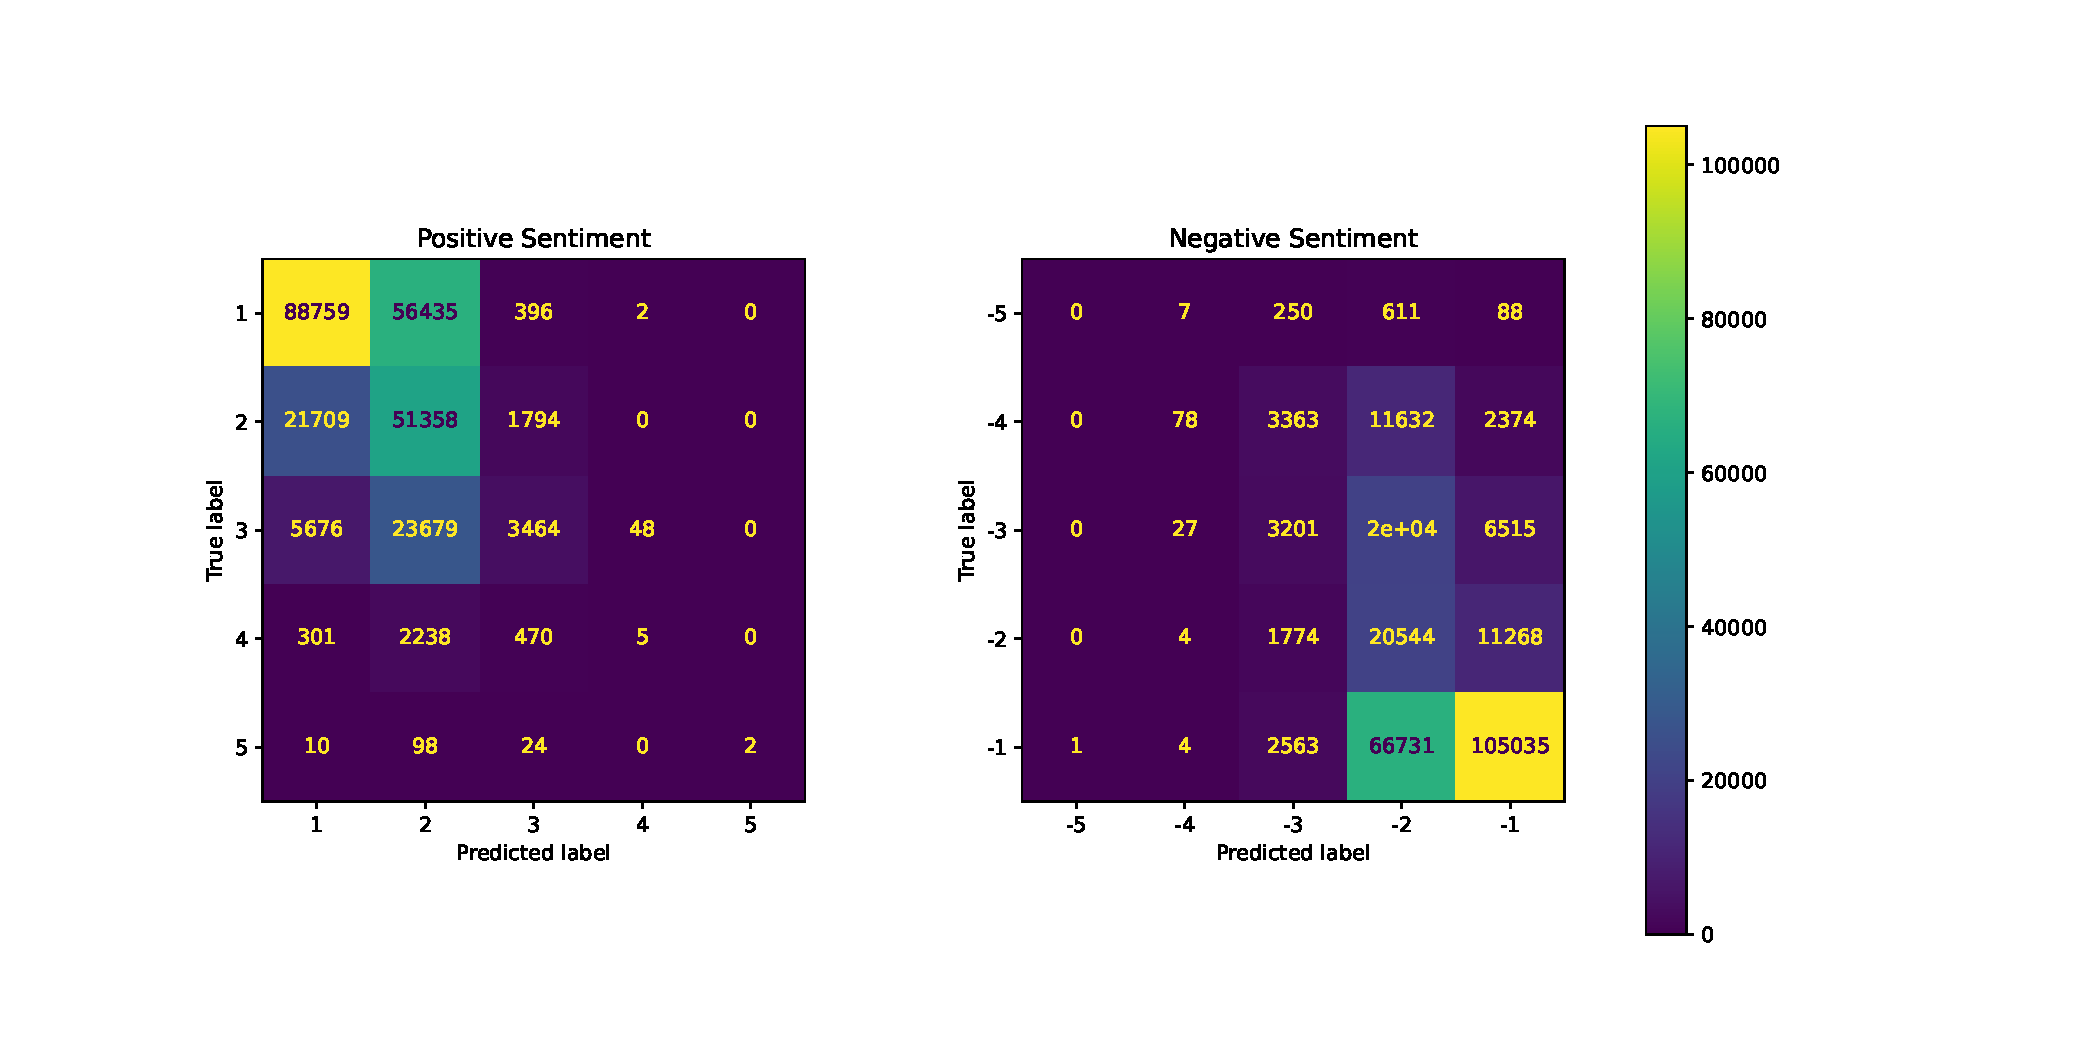
\includegraphics[width=\textwidth]{images/grad_boost_av_cbow.pdf}
        \caption{Confusion matrix for the Gradient Boosting 'classifier' trained on CBOW-embeddings that were aggregated by averaging.}    
        \label{fig:grad_boost_av_cbow}
    \end{subfigure}
    \hfill
    \begin{subfigure}[b]{0.475\textwidth}
        \centering
        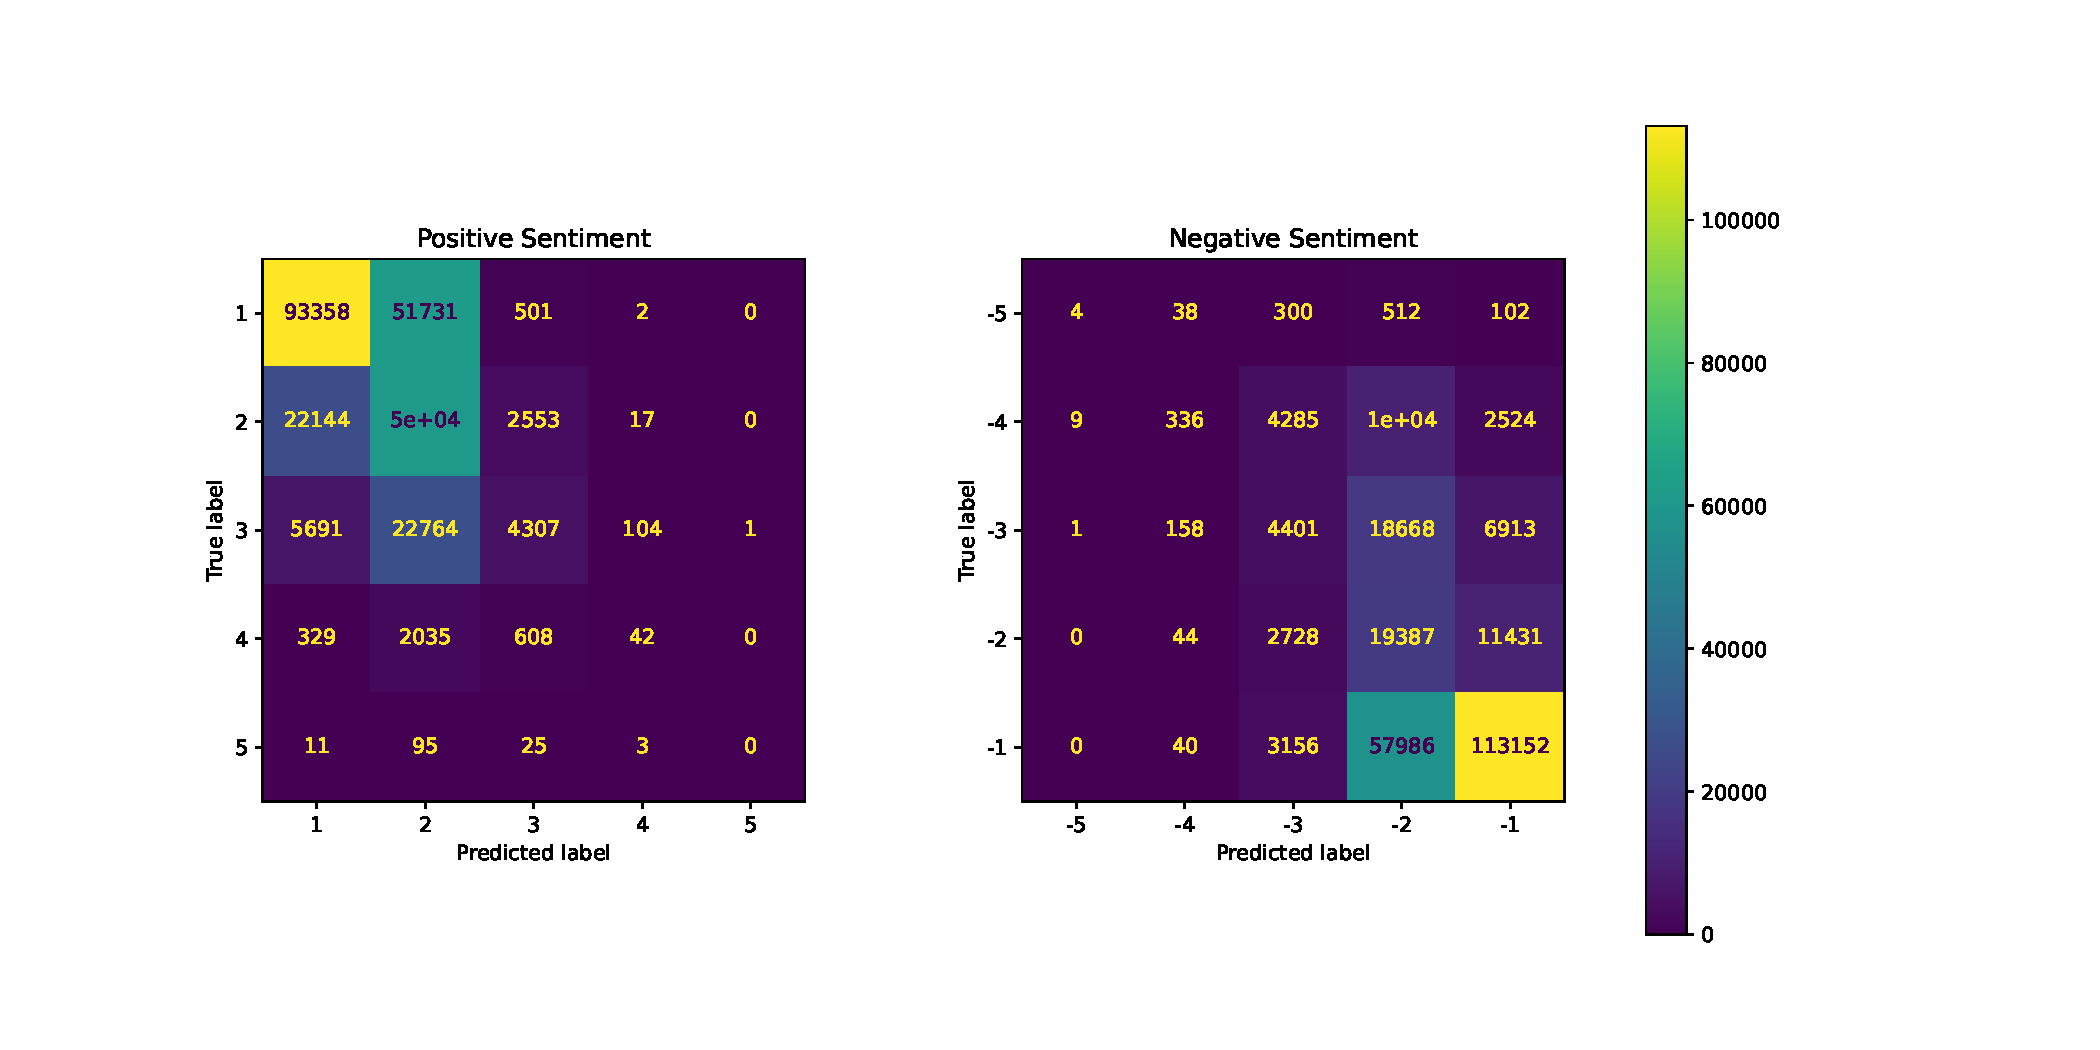
\includegraphics[width=\textwidth]{images/grad_boost_sum_cbow.pdf}
        \caption{Confusion matrix for the Gradient Boosting 'classifier' trained on CBOW-embeddings that were aggregated by summing.}    
        \label{fig:grad_boost_sum_cbow}
    \end{subfigure}
    \vskip\baselineskip
    \begin{subfigure}[b]{0.475\textwidth}
        \centering
        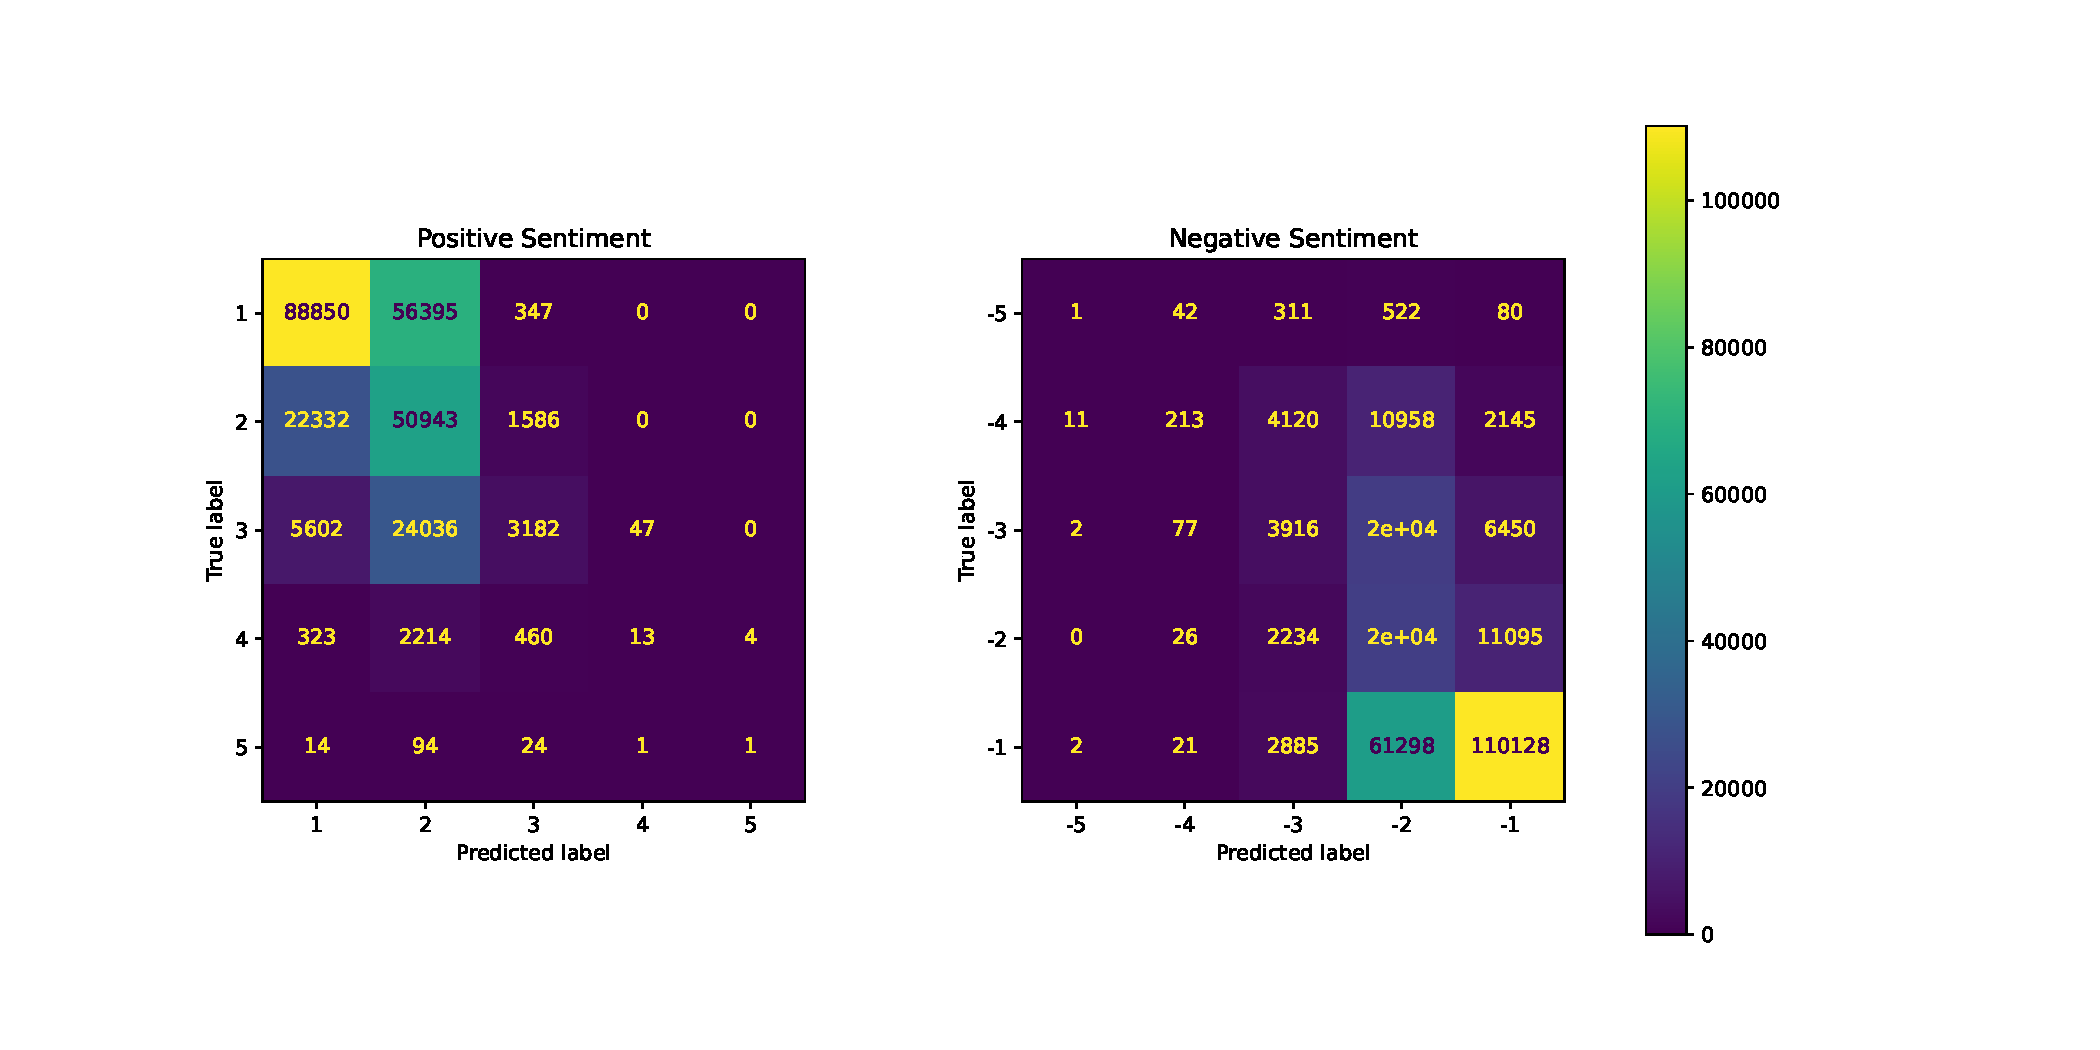
\includegraphics[width=\textwidth]{images/grad_boost_av_sgram.pdf}
        \caption{Confusion matrix for the Gradient Boosting 'classifier' trained on Skip-gram embeddings that were aggregated by averaging.}    
        \label{fig:grad_boost_av_sgram}
    \end{subfigure}
    \hfill
    \begin{subfigure}[b]{0.475\textwidth}
        \centering
        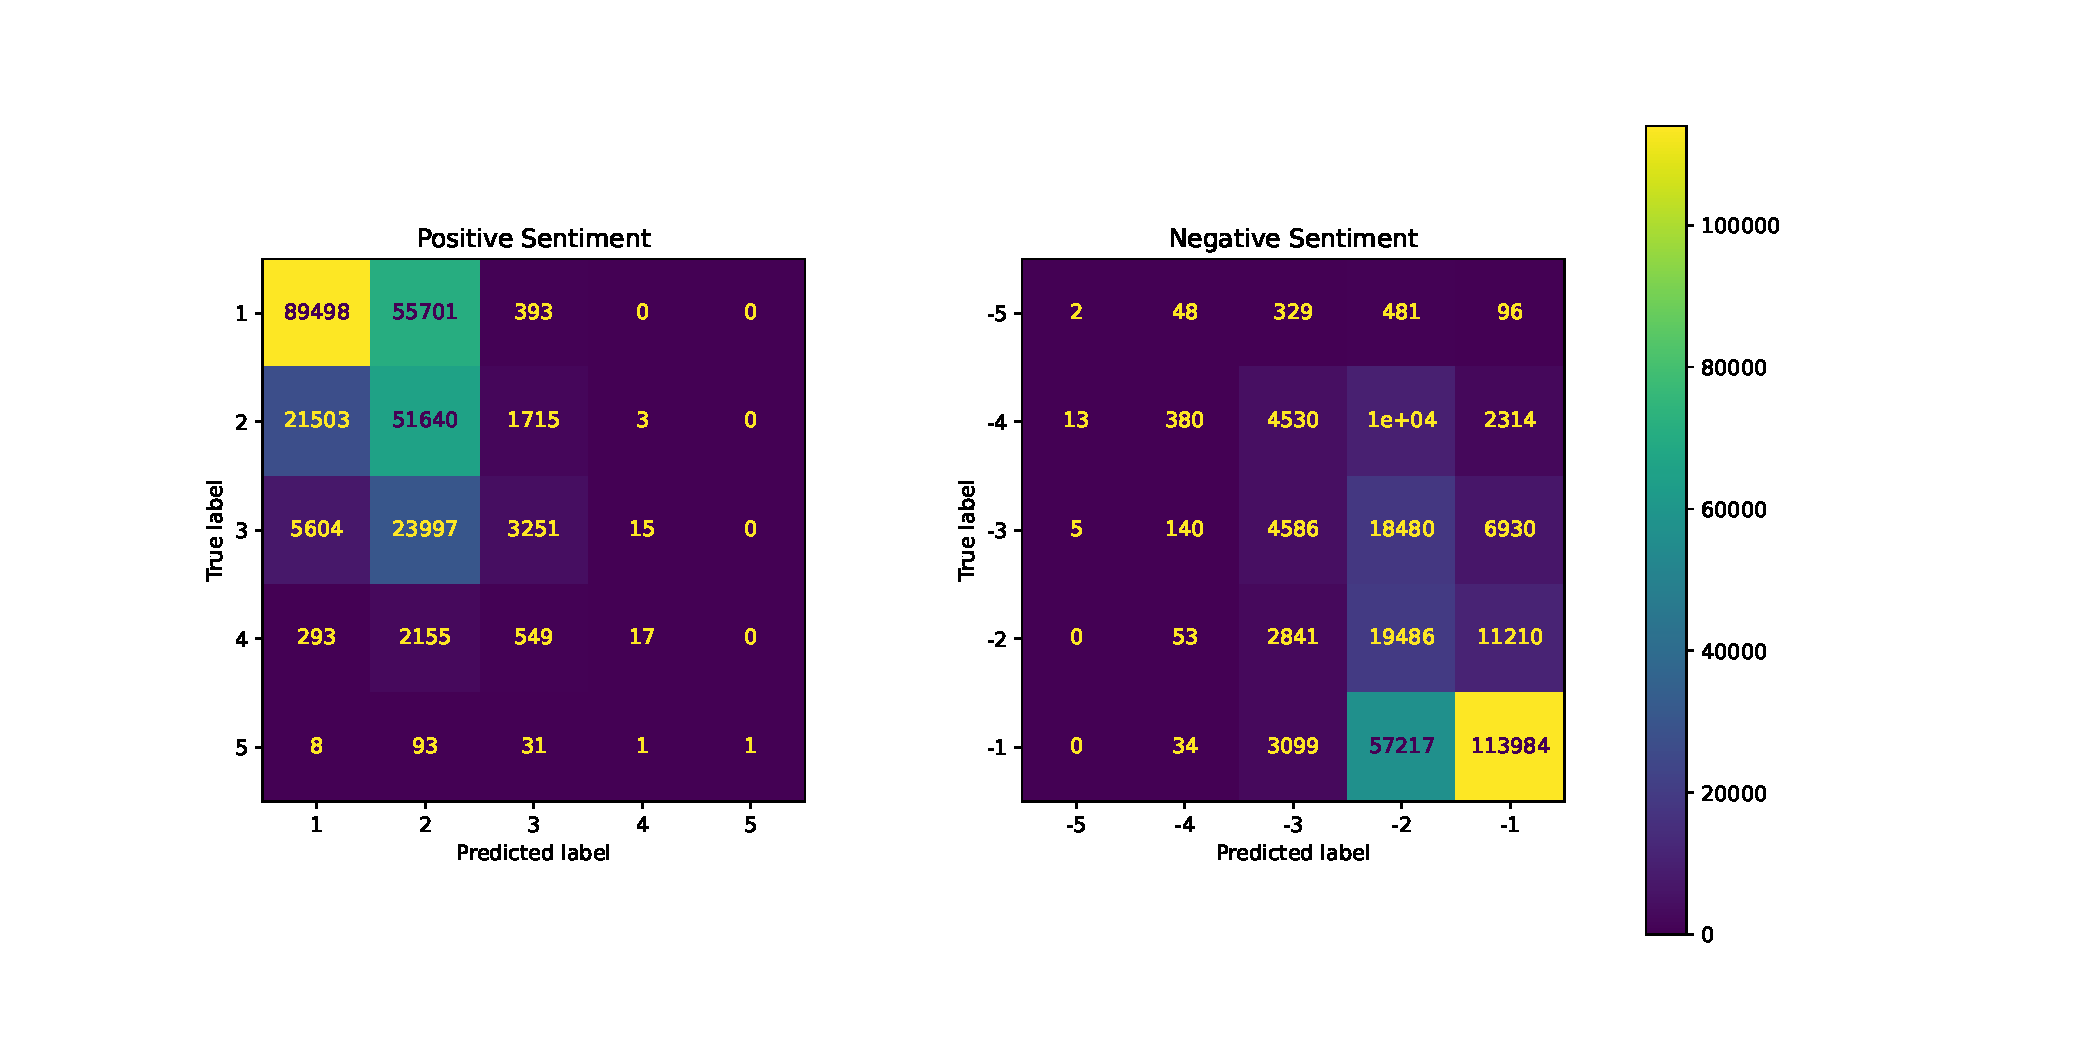
\includegraphics[width=\textwidth]{images/grad_boost_sum_sgram.pdf}
        \caption{Confusion matrix for the Gradient Boosting 'classifier' trained on Skip-gram embeddings that were aggregated by summing.}    
        \label{fig:grad_boost_sum_sgram}
    \end{subfigure}
   \vskip\baselineskip
    \begin{subfigure}[b]{0.475\textwidth}
        \centering
        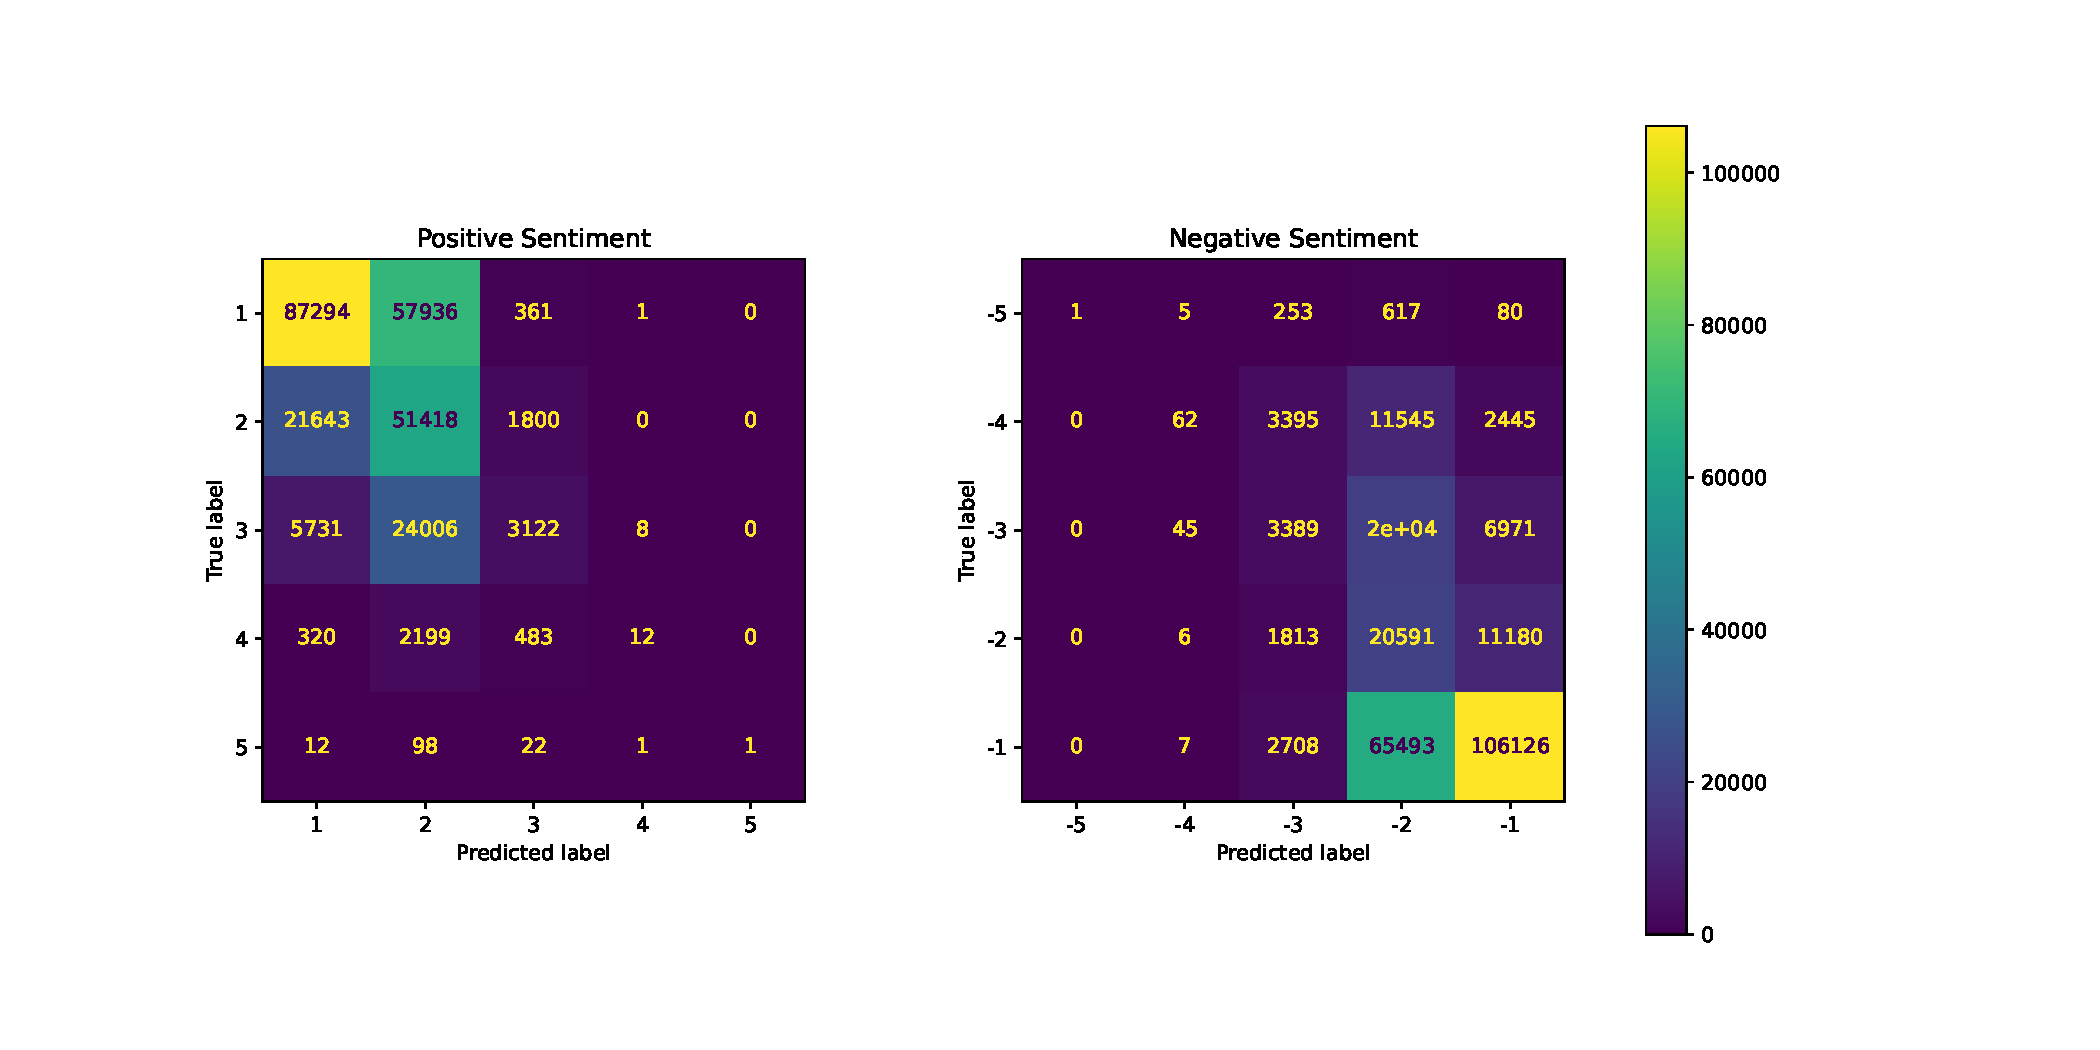
\includegraphics[width=\textwidth]{images/grad_boost_av_ft.pdf}
        \caption{Confusion matrix for the Gradient Boosting 'classifier' trained on FastText embeddings that were aggregated by averaging.}    
        \label{fig:grad_boost_av_ft}
    \end{subfigure}
    \hfill
    \begin{subfigure}[b]{0.475\textwidth}
        \centering
        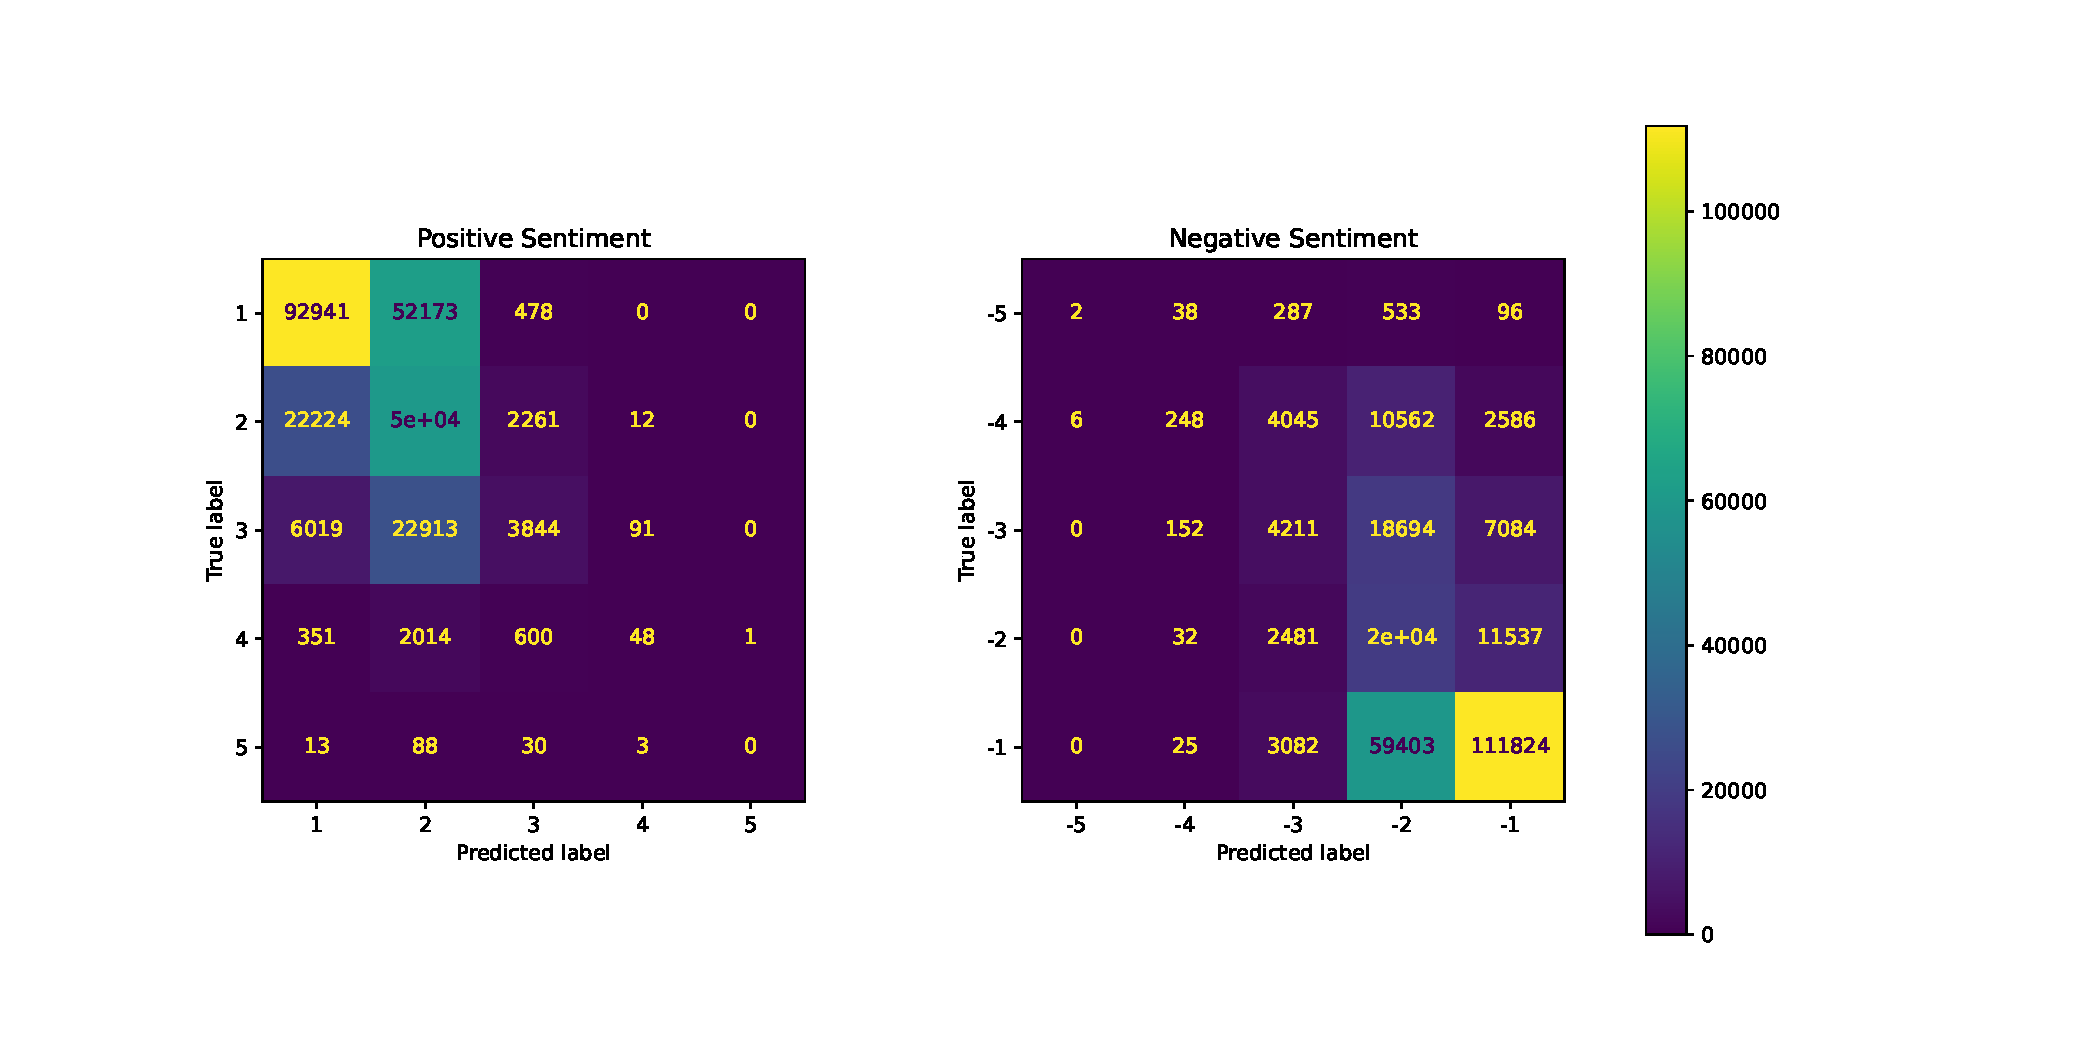
\includegraphics[width=\textwidth]{images/grad_boost_sum_ft.pdf}
        \caption{Confusion matrix for the Gradient Boosting 'classifier' trained on FastText embeddings that were aggregated by summing.}    
        \label{fig:grad_boost_sum_ft}
    \end{subfigure}
    \caption{Confusion matrices of six models trained with the Gradient Boosting algorithm. The models were selected based on a cutoff of $\ge 0.54$ for the training score (weighted harmonic F1 score).} 
    \label{fig:confusion_gensim}
\end{figure*}


\begin{figure*}
    \centering
    \begin{subfigure}[b]{0.475\textwidth}
        \centering
        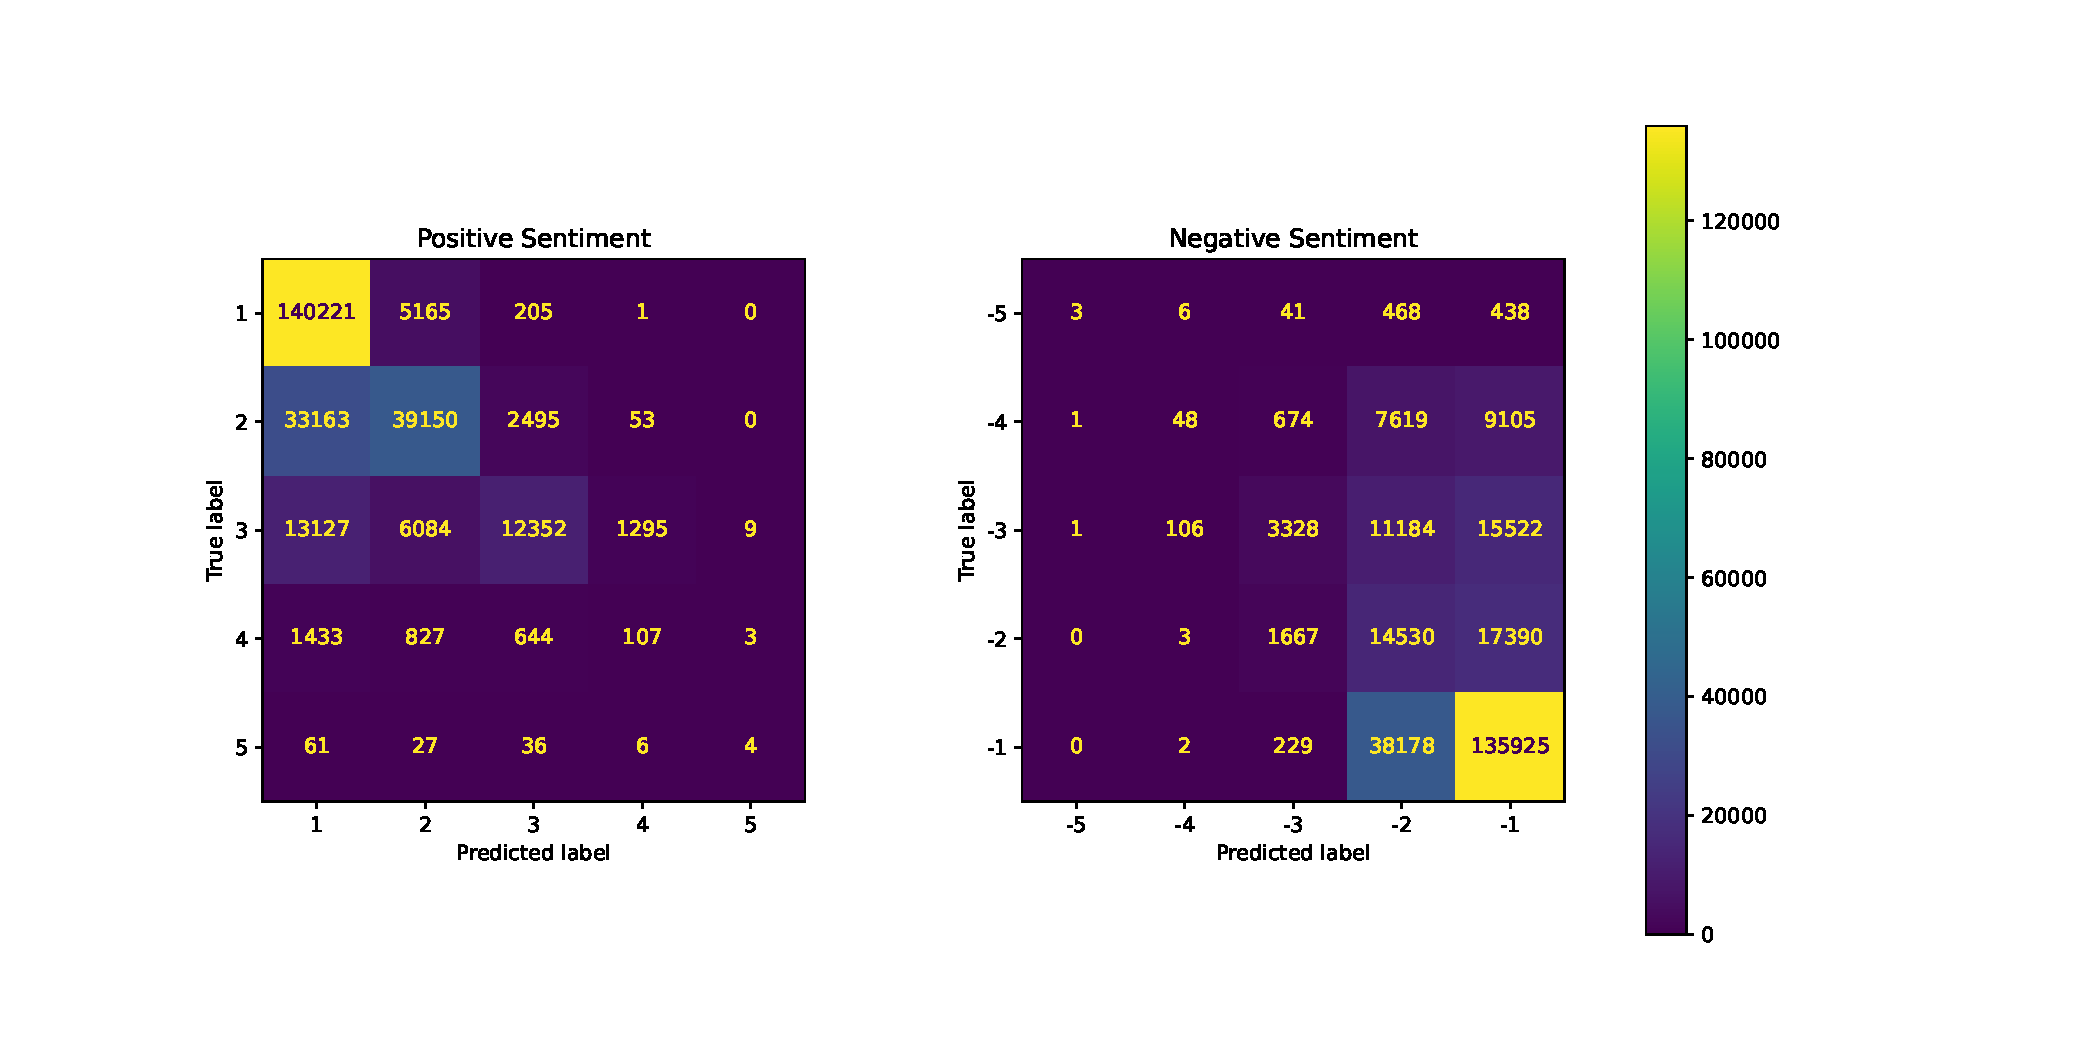
\includegraphics[width=\textwidth]{images/grad_boost_av_bow.pdf}
        \caption{Confusion matrix for the Gradient Boosting 'classifier' trained on BoW-embeddings that were aggregated by averaging.}    
        \label{fig:grad_boost_av_bow}
    \end{subfigure}
    \hfill
    \begin{subfigure}[b]{0.475\textwidth}
        \centering
        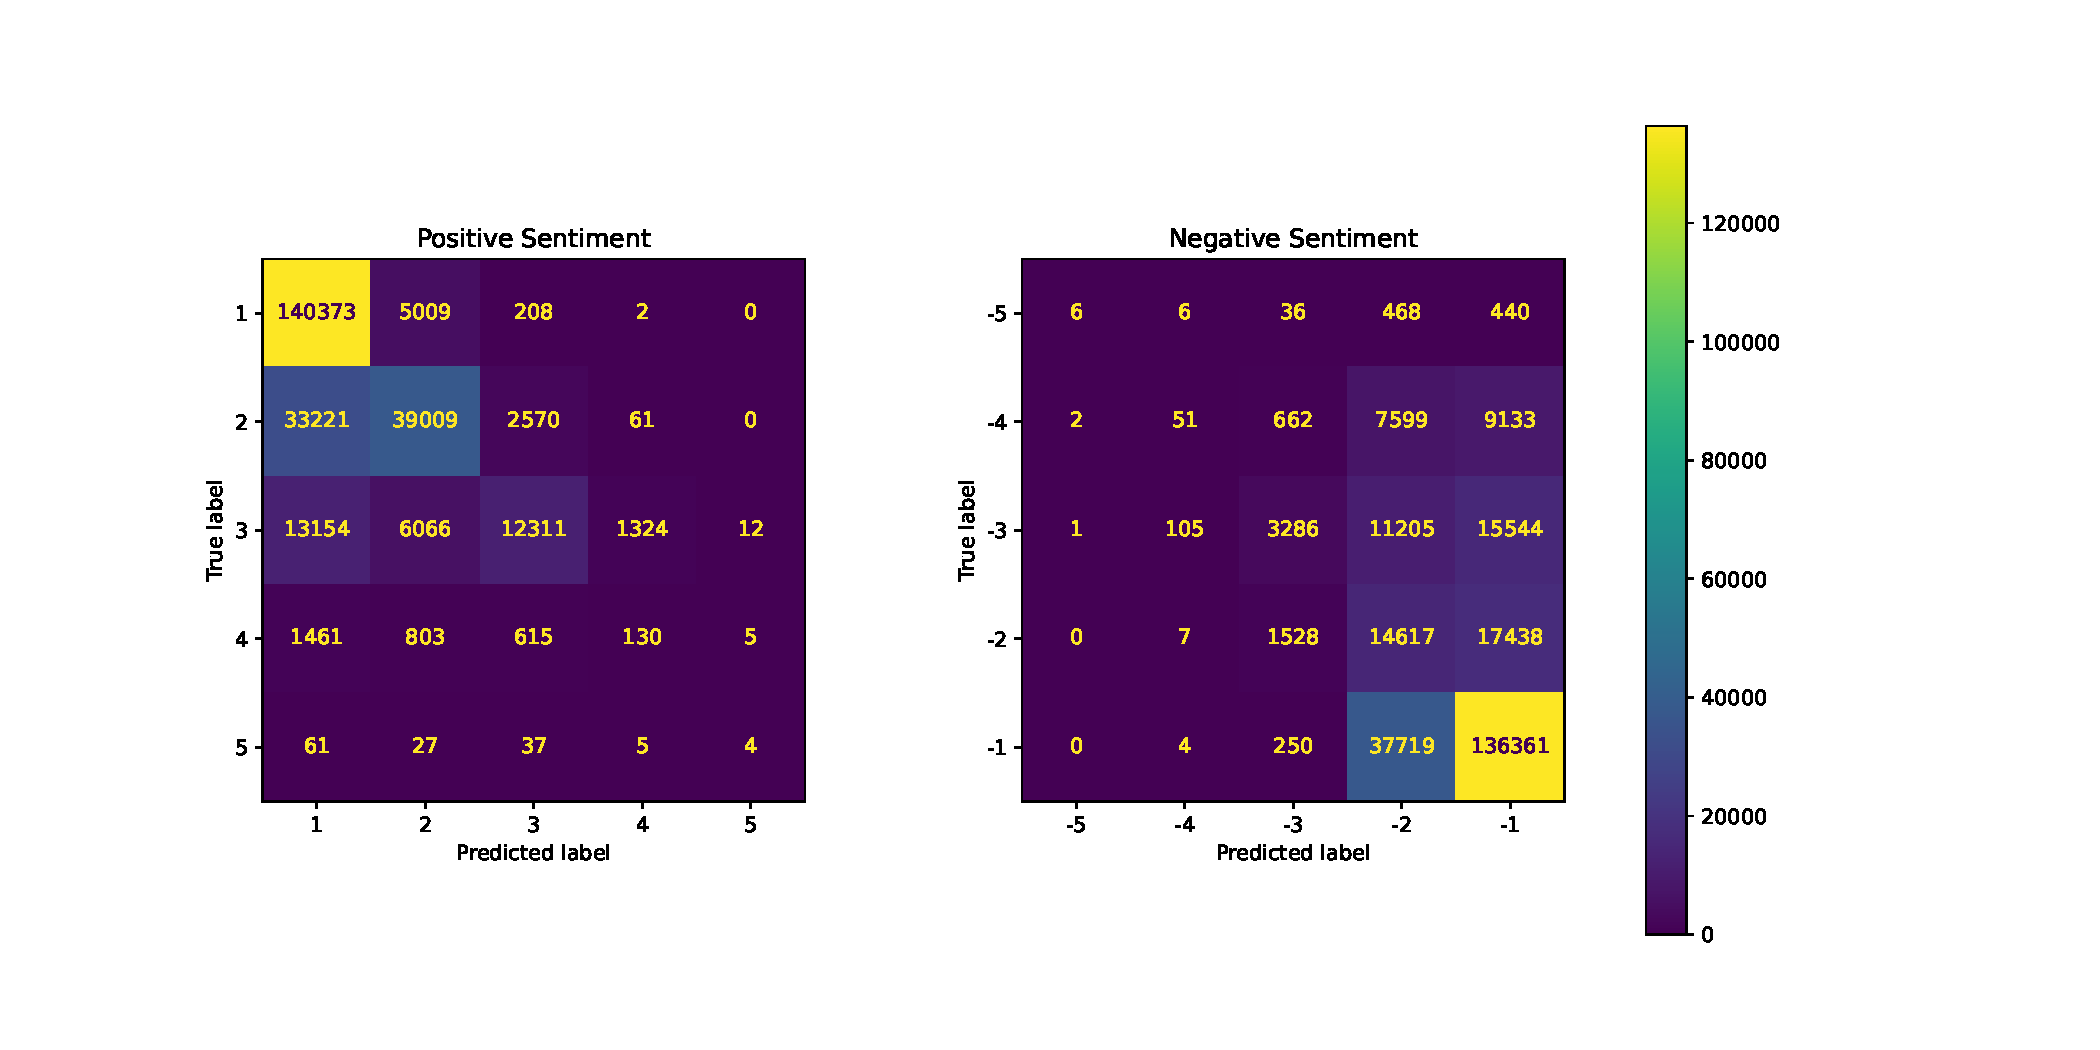
\includegraphics[width=\textwidth]{images/grad_boost_av_tfidf.pdf}
        \caption{Confusion matrix for the Gradient Boosting 'classifier' trained on TF-IDF-embeddings that were aggregated by averaging.}    
        \label{fig:grad_boost_av_tfidf}
    \end{subfigure}
    \vskip\baselineskip
    \begin{subfigure}[b]{0.475\textwidth}
        \centering
        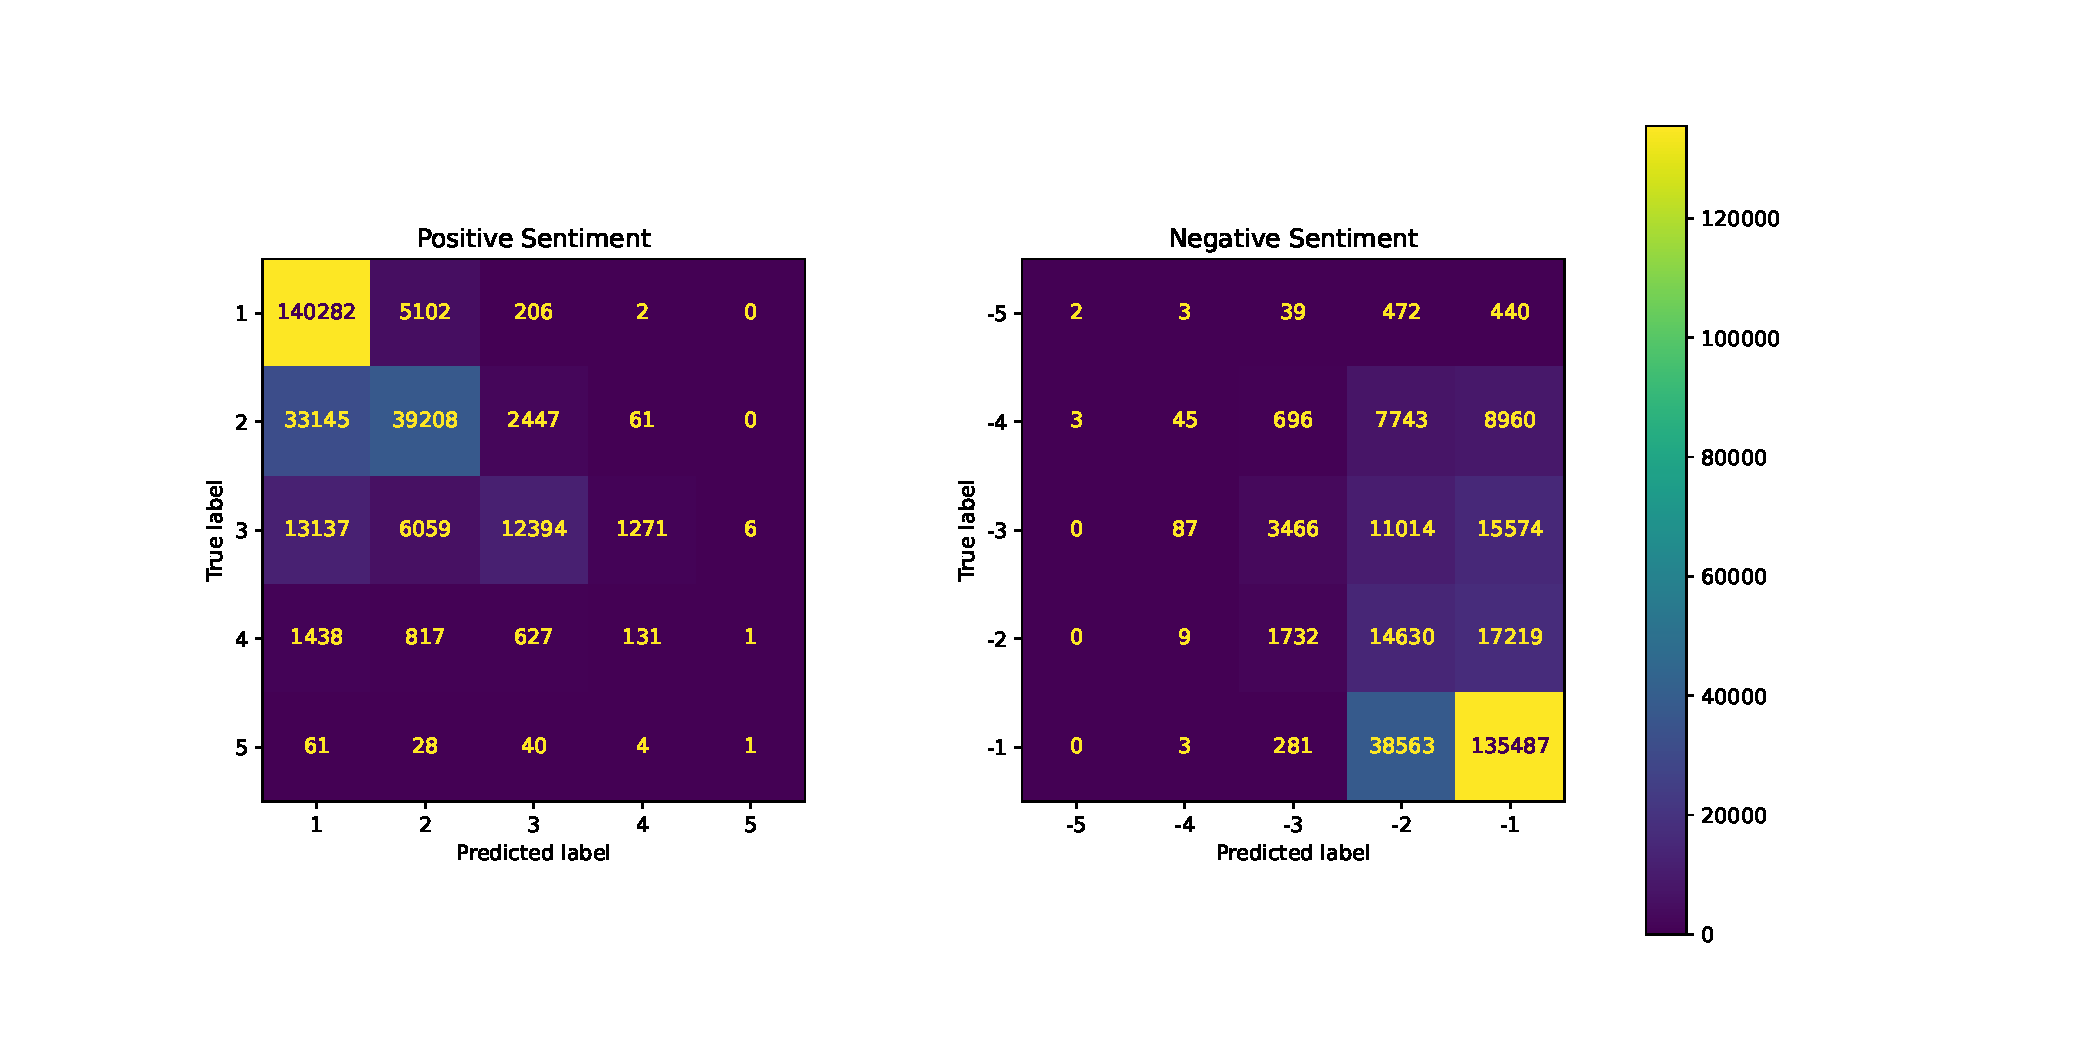
\includegraphics[width=\textwidth]{images/grad_boost_sum_bow.pdf}
        \caption{Confusion matrix for the Gradient Boosting 'classifier' trained on BoW-embeddings that were aggregated by summing.}    
        \label{fig:grad_boost_sum_bow}
    \end{subfigure}
    \hfill
    \begin{subfigure}[b]{0.475\textwidth}
        \centering
        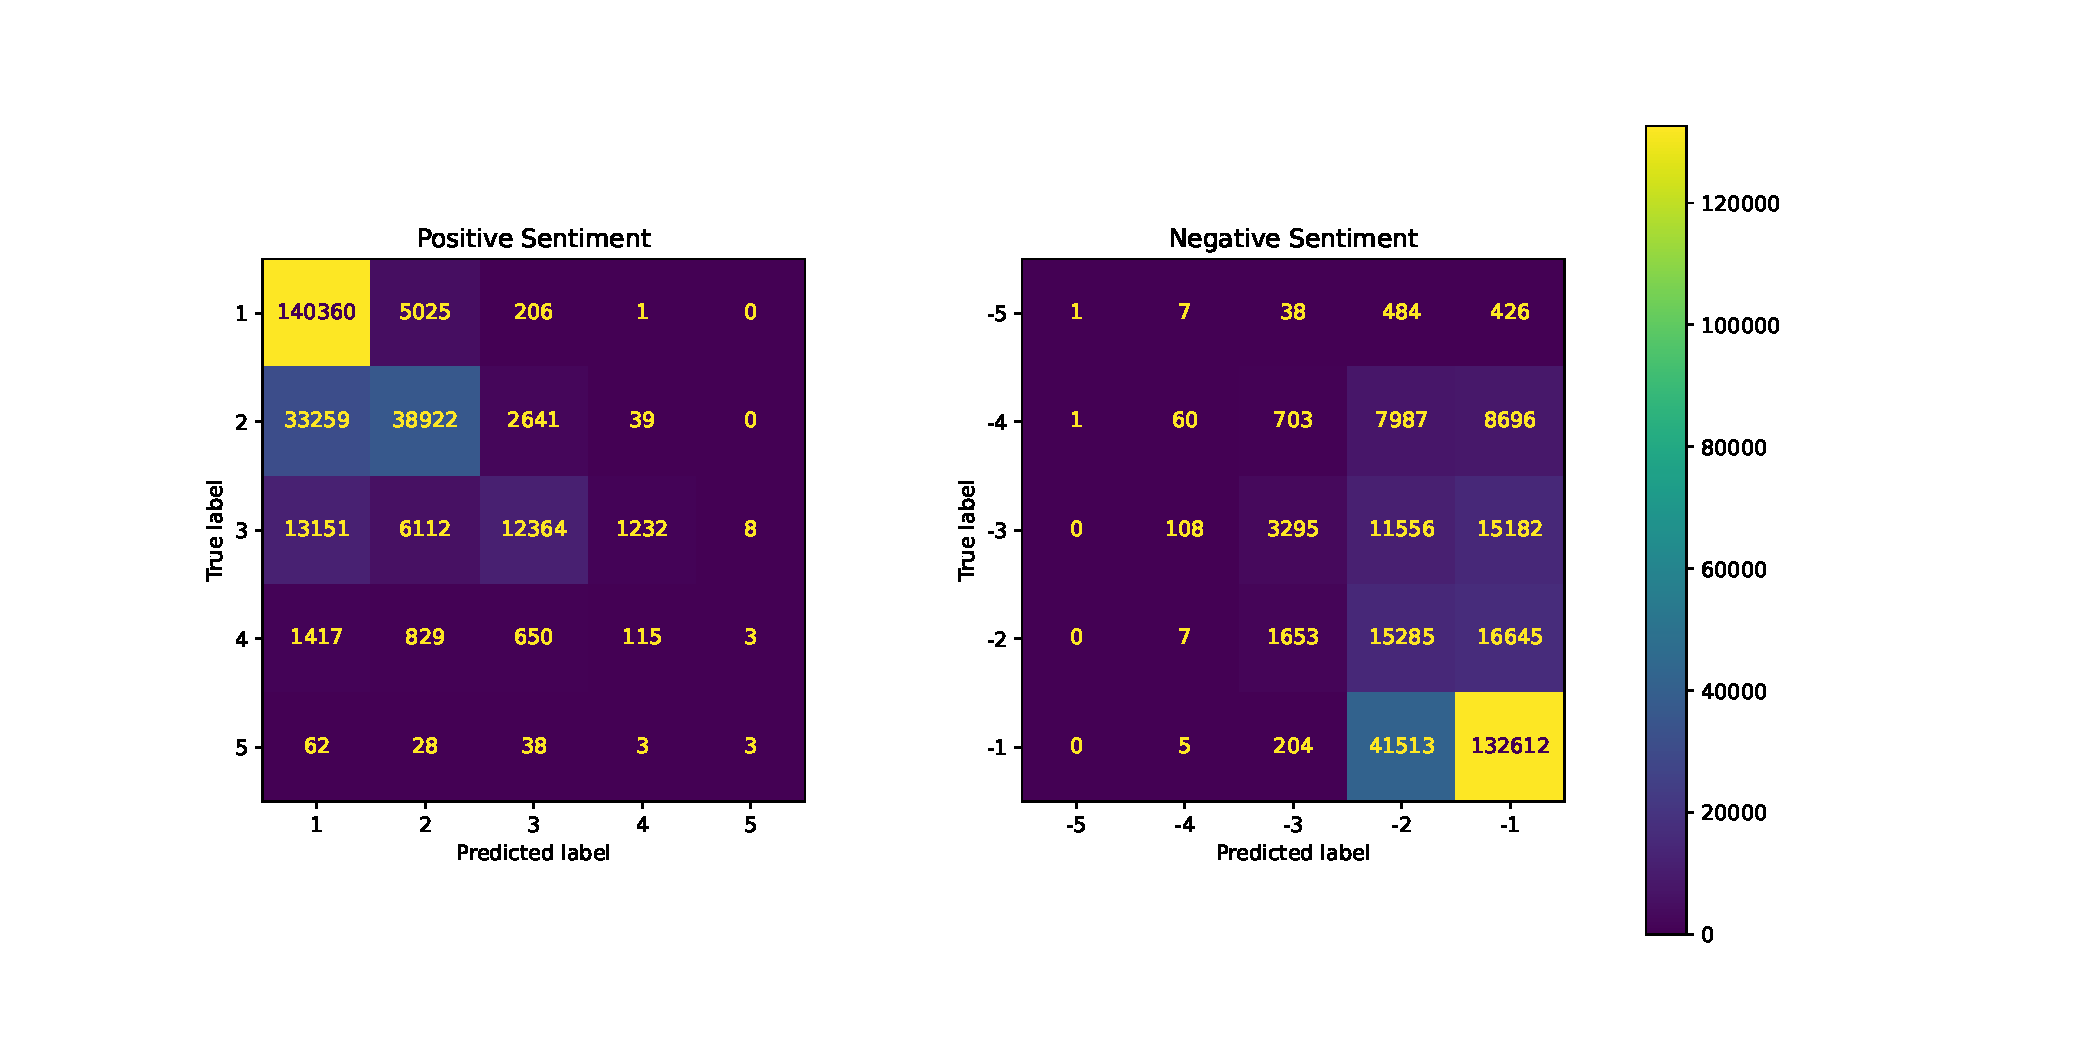
\includegraphics[width=\textwidth]{images/grad_boost_sum_tfidf.pdf}
        \caption{Confusion matrix for the Gradient Boosting 'classifier' trained on TF-IDF embeddings that were aggregated by summing.}    
        \label{fig:grad_boost_sum_tfidf}
    \end{subfigure}
   \vskip\baselineskip
    \begin{subfigure}[b]{0.475\textwidth}
        \centering
        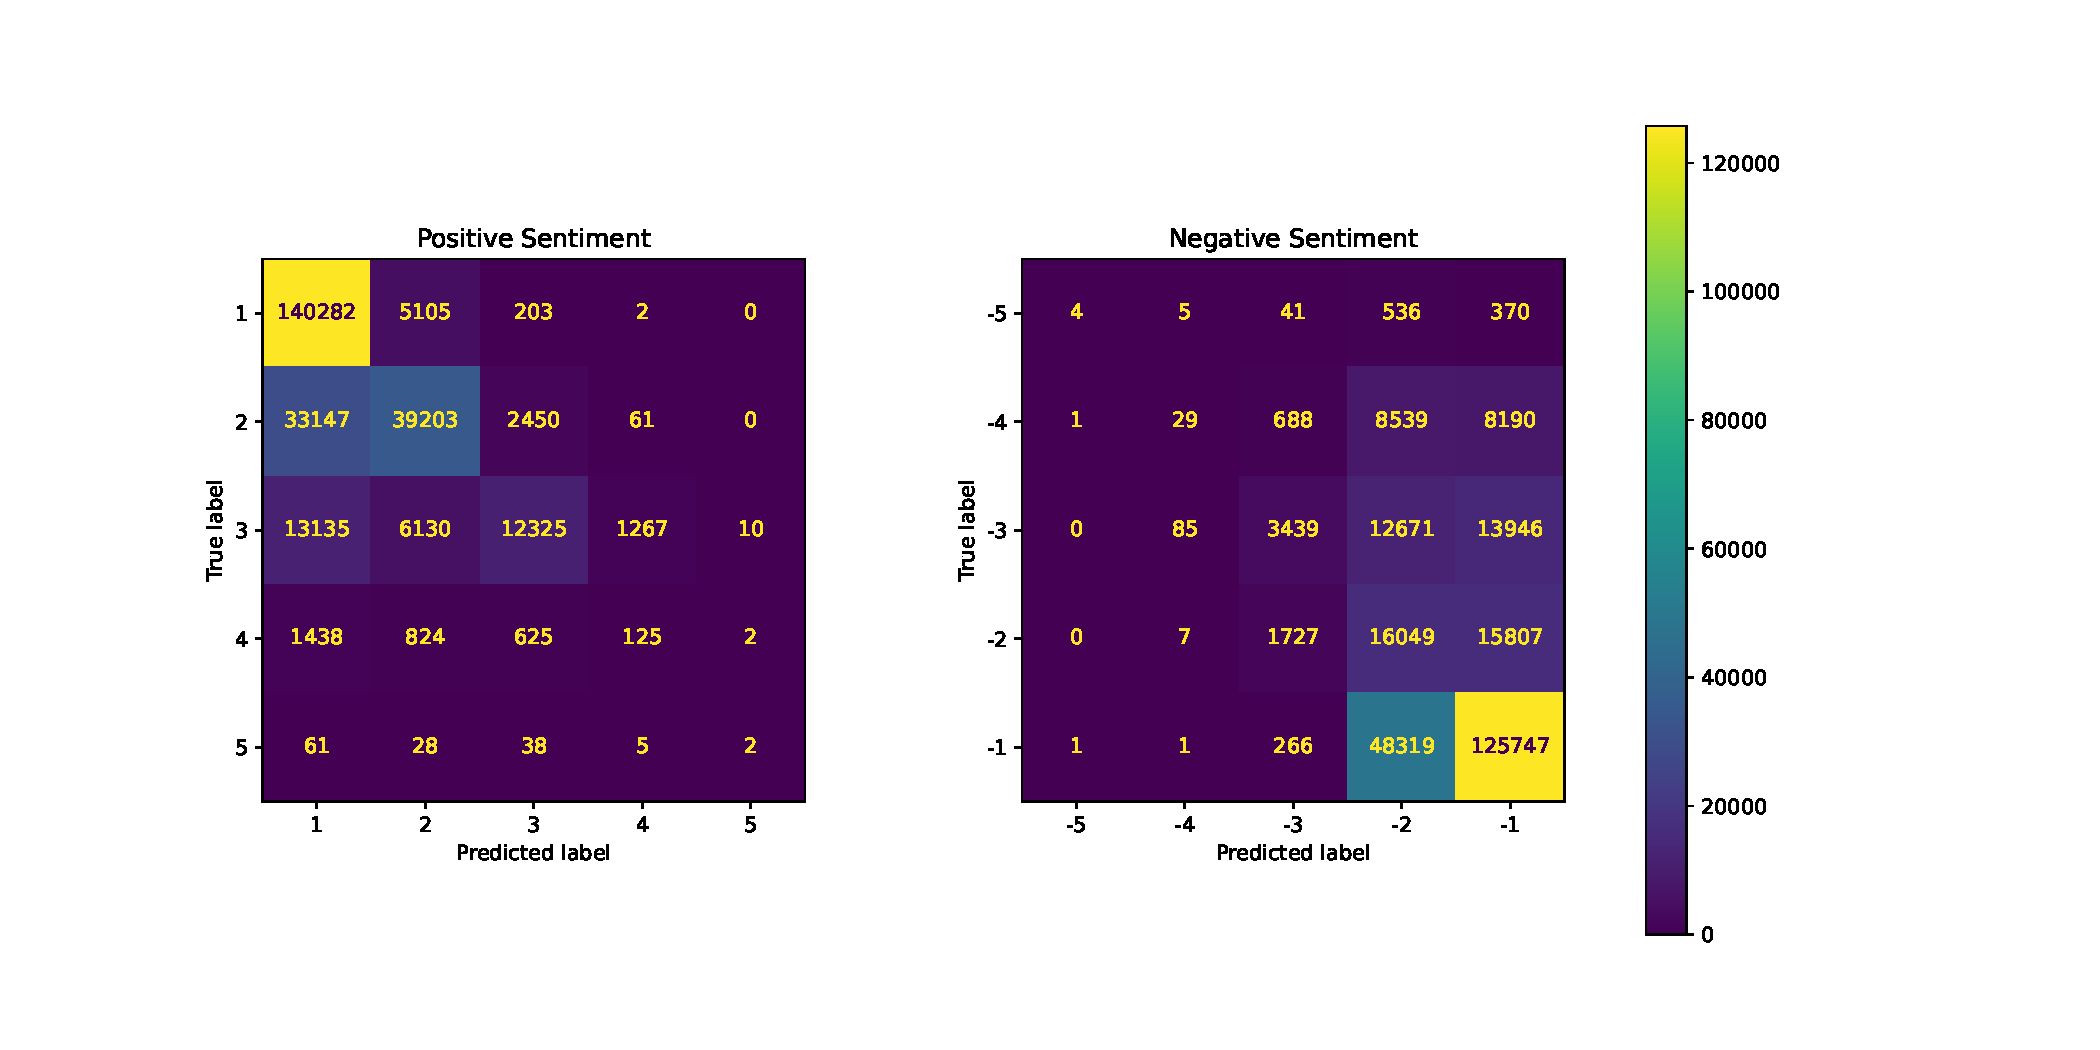
\includegraphics[width=\textwidth]{images/grad_boost_mm_bow.pdf}
        \caption{Confusion matrix for the Gradient Boosting 'classifier' trained on BoW-embeddings that were aggregated by concatenating the minimum and maximum over all word embeddings.}    
        \label{fig:grad_boost_mm_bow}
    \end{subfigure}
    \hfill
    \begin{subfigure}[b]{0.475\textwidth}
        \centering
        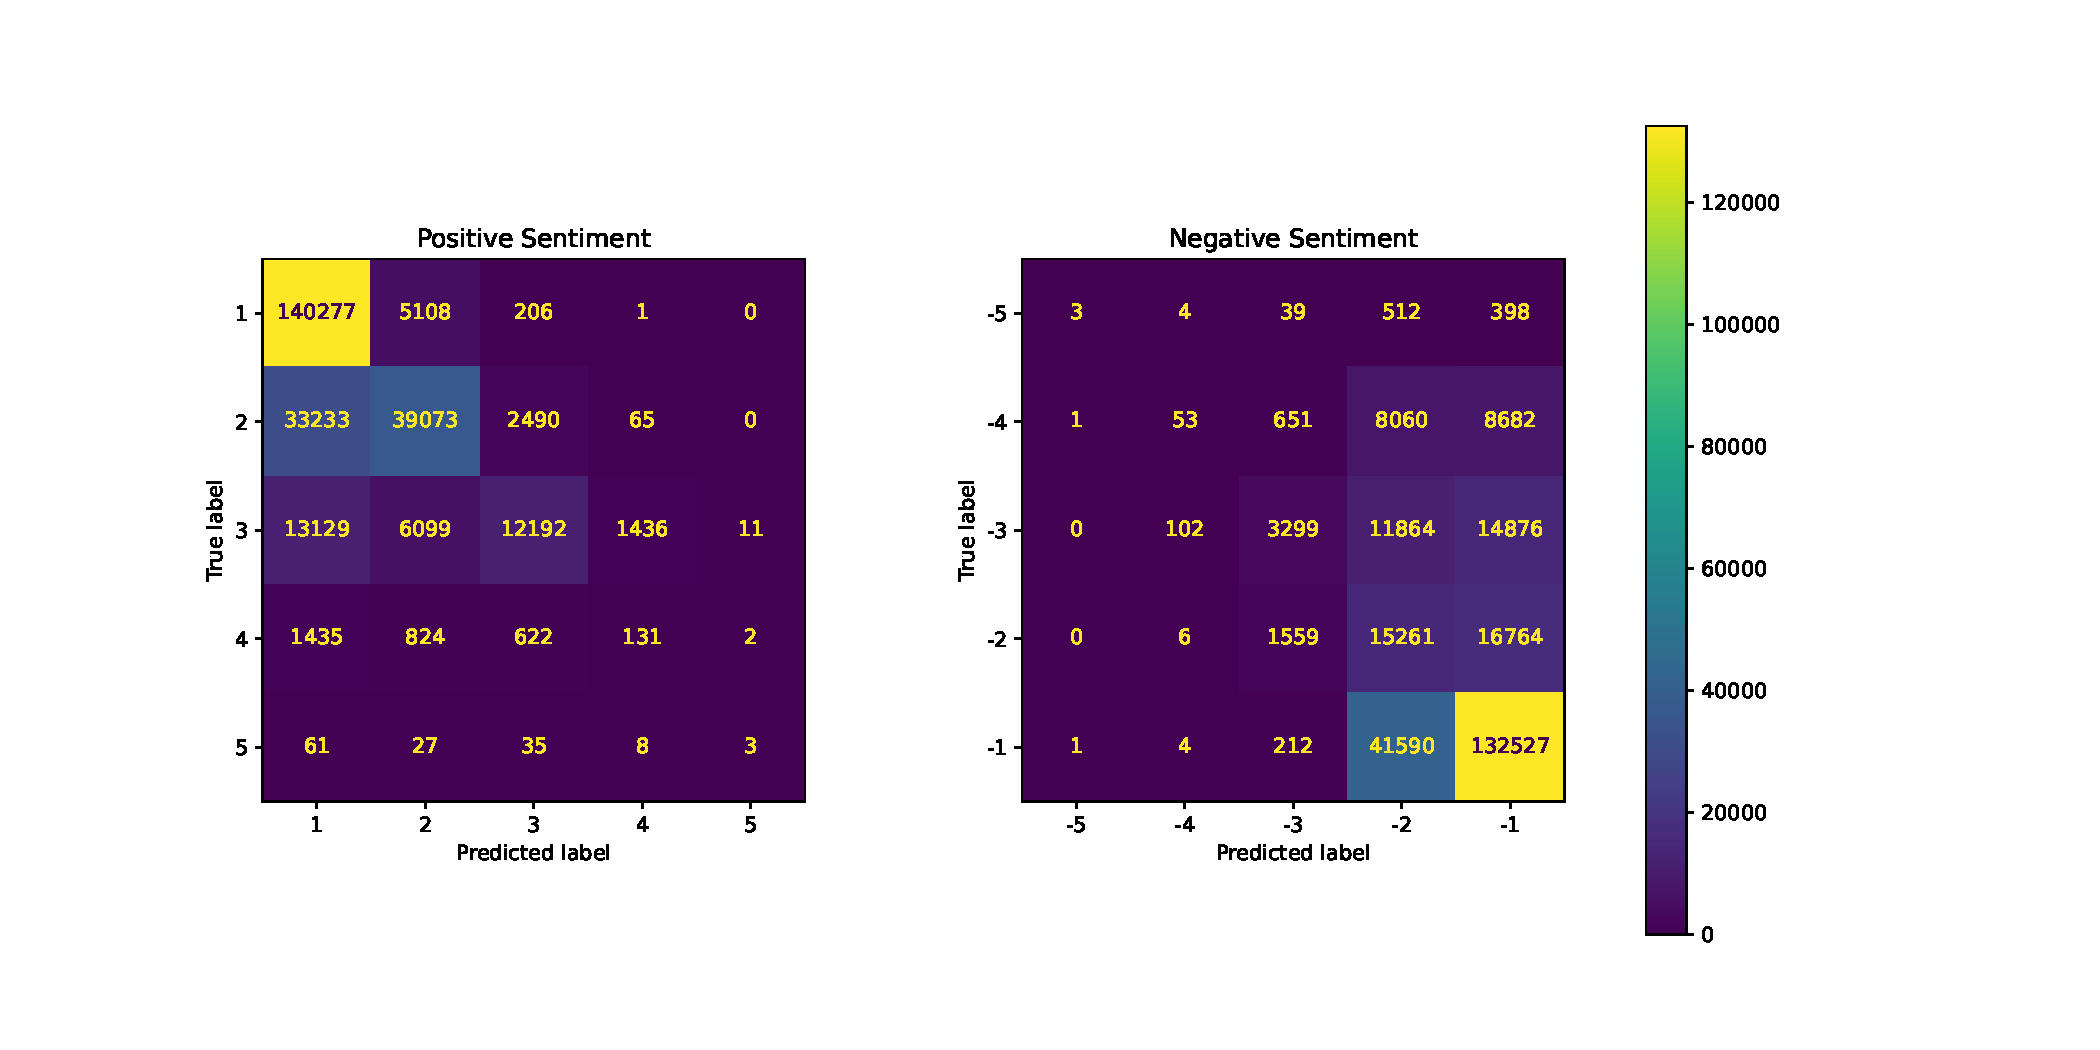
\includegraphics[width=\textwidth]{images/grad_boost_mm_tfidf.pdf}
        \caption{Confusion matrix for the Gradient Boosting 'classifier' trained on TF-IDF-embeddings that were aggregated by concatenating the minimum and maximum over all word embeddings.}
        \label{fig:grad_boost_mm_tfidf}
    \end{subfigure}
    \caption{Confusion matrices of six models trained with the Gradient Boosting algorithm. The models were selected based on a cutoff of $\ge 0.54$ for the training score (weighted harmonic F1 score).} 
    \label{fig:confusion_sklearn}
\end{figure*}

If we look at the confusion matrices of the models that have a final training score of $\ge 0.54$ (Figures \ref{fig:confusion_gensim} and \ref{fig:confusion_sklearn}), we see that (likely due to class imbalance), very positive and very negative tweets get misclassified most often. Therefore, we would like a model that prevents this somewhat.
Our final choice, taking our computational restrictions into account, is therefore to use TF-IDF for word embedding, averaging or summing as aggregation method, and Gradient Boosting as the training method. Although not the fastest, both these options strongly outperform most of the other models, even though the vocabulary size is limited.
Since OOV words cannot be accounted for with TF-IDF, a Gradient Boosting model trained with FastText embeddings aggregated by summing might still perform reasonably, and is thus considered a strong runner up for our final choice, especially since the vector size was limited in the embedding model.

As mentioned in the previous paragraph, one major thing we limited, was the final vector size of our embedding models. This was done to facilitate training. Still, for the Gensim models, the vector size we chose (v=20) vastly differs from the ones mentioned in the original papers (v=300), so using a larger vector size can potentially improve our results. The same holds for vocabulary size in the TF-IDF and BoW models, which we set at v=250. We expect some classifier results to improve when using larger feature vectors as input for the classification model.

In addition, we could try to train our very own convolutional neural network (CNN) for sentiment classification, which gives us much more flexibility than the usage of predefined models from existing libraries like scikit-learn.

Finally, we could look into classification vs. regression more in depth, and compare how 'real' classifiers perform, which would be especially useful to correct for class imbalance.
